\documentclass[11pt,class=report,crop=false]{standalone}
\usepackage[screen]{../python}


\begin{document}

%====================================================================
\chapitre{Big data II}
%====================================================================

\index{big data@\emph{big data}}


\objectifs{L'essor des \emph{big-data} et de l'intelligence artificielle est dû à l'apparition de nouveaux algorithmes adaptés à la résolution de problèmes complexes : reconnaissance d'images, comportement des électeurs, conduite autonome de voitures\ldots{} Dans cette seconde partie tu vas programmer quelques algorithmes emblématiques et innovants.}

\bigskip


%%%%%%%%%%%%%%%%%%%%%%%%%%%%%%%%%%%%%%%%%%%%%%%%%%%%%%%%%%%%%%%%
%%%%%%%%%%%%%%%%%%%%%%%%%%%%%%%%%%%%%%%%%%%%%%%%%%%%%%%%%%%%%%%%

\begin{cours}[Les $k$ voisins les plus proches]

Considérons un électeur qui ne sait pas pour qui voter. 
Il décide donc de voter comme ses voisins !

\myfigure{0.5}{
	\tikzinput{fig_voisins_1a}
}

Pour modéliser la situation, on considère d'abord des points du plan qui peuvent être de deux types, soit des carrés bleus, soit des ronds rouges, on appelle ces points les \emph{points de référence}.
Ces points représentent les personnes qui savent déjà pour qui elles vont voter (parmi le choix rouge/bleu).
Les autres points n'ont pas encore de couleur, cela représente toutes les personnes qui ne savent pas pour qui elles vont voter.

Voici comment les indécis se décident : 
pour chaque point non colorié, on regarde le point de référence le plus proche, on colorie alors le point par la couleur de ce point de référence.

\myfigure{0.5}{
	\tikzinput{fig_voisins_1b}
	\tikzinput{fig_voisins_1c}
}

On généralise cette procédure avec la notion de \og{}$k$ voisins\fg{}.
Soit $k$ un entier positif. Pour un point non colorié, on cherche
les $k$ points de référence les plus proches (ce sont les $k$ voisins). La couleur attribuée est la couleur majoritaire de ces $k$ voisins.

Sur l'exemple ci-dessous, les $k=3$ voisins sont formés de $2$ ronds rouges et $1$ carré bleu. On colorie donc l'étoile en rouge.
\myfigure{0.5}{
	\tikzinput{fig_voisins_1d}	
}

Le but de l'activité suivante est de colorier tous les points d'une zone grâce à cette méthode.
\end{cours}


%%%%%%%%%%%%%%%%%%%%%%%%%%%%%%%%%%%%%%%%%%%%%%%%%%%%%%%%%%%%%%%%
% Activité 1 - Les k voisins les plus proches
%%%%%%%%%%%%%%%%%%%%%%%%%%%%%%%%%%%%%%%%%%%%%%%%%%%%%%%%%%%%%%%%

\begin{activite}[Les $k$ voisins les plus proches]
	
\objectifs{Objectifs : colorier un point en fonction de la couleur de ses voisins.}


\begin{enumerate}
	\item \textbf{Préparation.}
	Programme des fonctions qui permettent d'afficher des points en couleur.
	On définit un point coloré, appelé \emph{cpoint}, par $(x,y,c)$
	où $x$ et $y$ sont des entiers avec $x_{\min} \le x \le x_{\max}$ et $y_{\min} \le y \le y_{\max}$
	et $c$ représente la couleur : $c=0$ pour du rouge et $c=1$ pour du bleu.
	
	
	\begin{enumerate}
		\item Définis des constantes globales \ci{xmin}, \ci{xmax}, \ci{ymin}, \ci{ymax} (par exemple $0$, $10$, $0$, $10$) pour la fenêtre des points.
		Programme une fonction \ci{afficher_cpoints(cpoints)} qui affiche une liste de cpoints.
		Par exemple pour \ci{cpoints = [(2,3,0),(5,7,1)]} cette fonction affiche un point en $(2,3)$ en rouge et un point en $(5,7)$ en bleu (figure de gauche).
		
		\begin{center}
			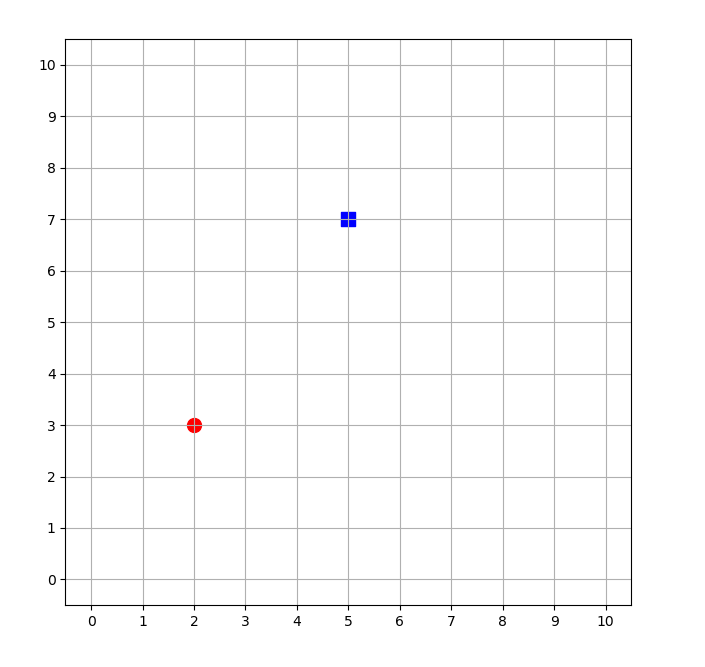
\includegraphics[scale=\myscale,scale=0.25]{ecran-voisins-1} \quad
			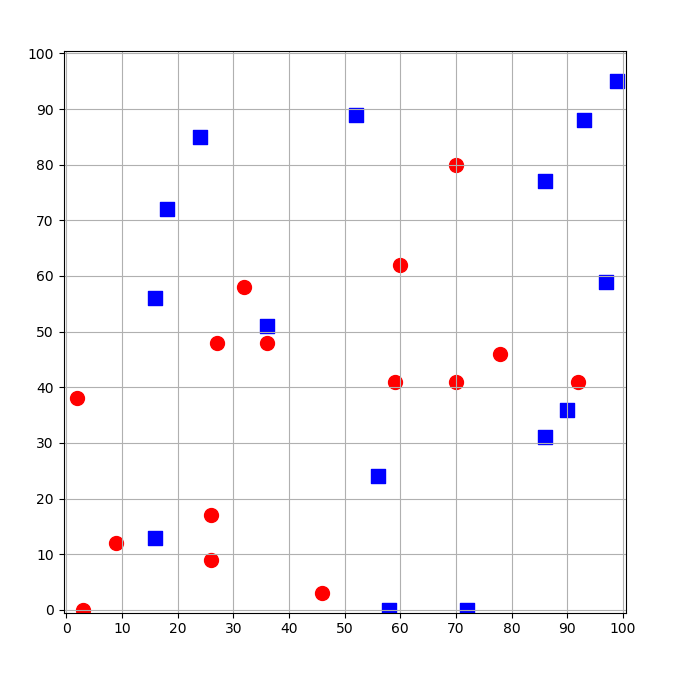
\includegraphics[scale=\myscale,scale=0.25]{ecran-voisins-2}
		\end{center}
		
		\item Programme une fonction \ci{fonction_couleur(x,y)} qui renvoie une couleur ($0$ ou $1$) pour un point $(x,y)$.
		Tu pourras essayer plusieurs fonctions :
		\begin{itemize}
			\item $0$ ou $1$ au hasard,
			\item $0$ si $((x^2+y^2)\% 100)  - 50>0$ \  et \  $1$ sinon,
			\item $0$ ou $1$ selon le signe de $\left(x-\frac{x_{\max}}{2}\right)^3 - 3 \left(x-\frac{x_{\max}}{2}\right)\left(y-\frac{y_{\max}}{2}\right)^2 - x_{\max}$,
			\item ou toute autre fonction de ton invention\ldots
		\end{itemize} 
		
		\item Programme une fonction \ci{generer_cpoints(N)} qui renvoie une liste aléatoire de $N$ cpoints $(x,y,c)$ (utilise la fonction précédente pour calculer $c$).
		Sur la figure de droite ci-dessus on a affiché $30$ points sur $[0,100]\times [0,100]$.
		
	\end{enumerate}
	
	\item \textbf{Le voisin le plus proche.}
	\begin{enumerate}
		\item Programme une fonction \ci{distance(P,Q)} qui calcule la distance entre $P = (x_1,y_1)$ et $Q=(x_2,y_2)$ :
		$$d = \sqrt{(x_1-x_2)^2 + (y_1-y_2)^2}.$$
		
		\item Programme une fonction \ci{un_voisin_proche(P,cpoints)}
		qui à partir d'un point $P=(x_0,y_0)$ renvoie un cpoint $Q_c = (x,y,c)$ parmi ceux de la liste donnée  et qui est le plus proche possible de $P$.
		
		\emph{Indications.}
		\begin{itemize}
			\item Il peut y avoir plusieurs voisins à la même distance, la fonction en renvoie un, peu importe lequel.
			
			\item Commence par définir un réel $d_{\min}$ très grand (par exemple $d_{\min} = 1000$ ou mieux $d_{\min} = + \infty$ par \ci{dmin = inf} du module \ci{math}). Ensuite calcule la distance entre $P$ et chaque $Q_c$ de la liste et renvoie le plus proche.

		\end{itemize}
	
		Sur l'exemple suivant $P = (4,3)$\couleurnb{ (en noir)}{} a pour plus proche voisin $Q = (6,2)$\couleurnb{ (en bleu)}{} qui est à une distance $d = \sqrt{5}$.
		
		\begin{center}
		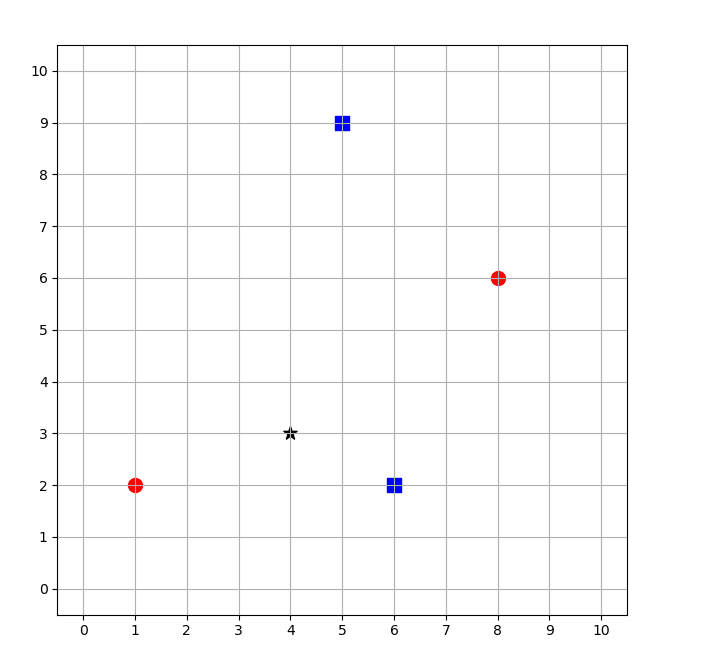
\includegraphics[scale=0.25]{ecran-voisins-3}
		\end{center}	

		
	\end{enumerate}
	
	\item \textbf{Coloriage.}
	\`A partir d'une liste de points colorés, on colorie tous les points : chaque point prend la couleur du voisin le plus proche. 	
	Programme ceci en une fonction \ci{colorier_par_un_voisin_proche(cpoints)}.
	
	Ci-dessous à gauche des points colorés initiaux et à droite le coloriage obtenu par la méthode du plus proche voisin. 
	\begin{center}
	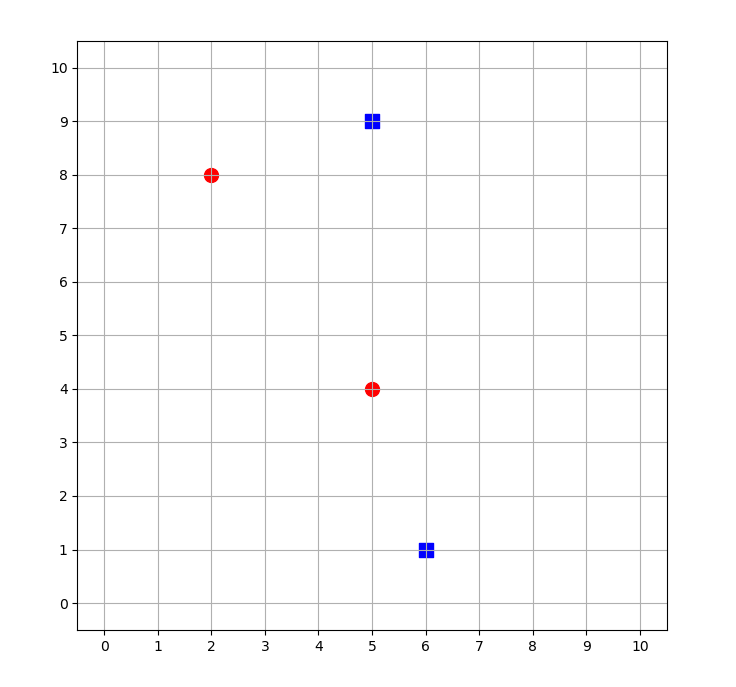
\includegraphics[scale=\myscale,scale=0.25]{ecran-voisins-4} \quad
	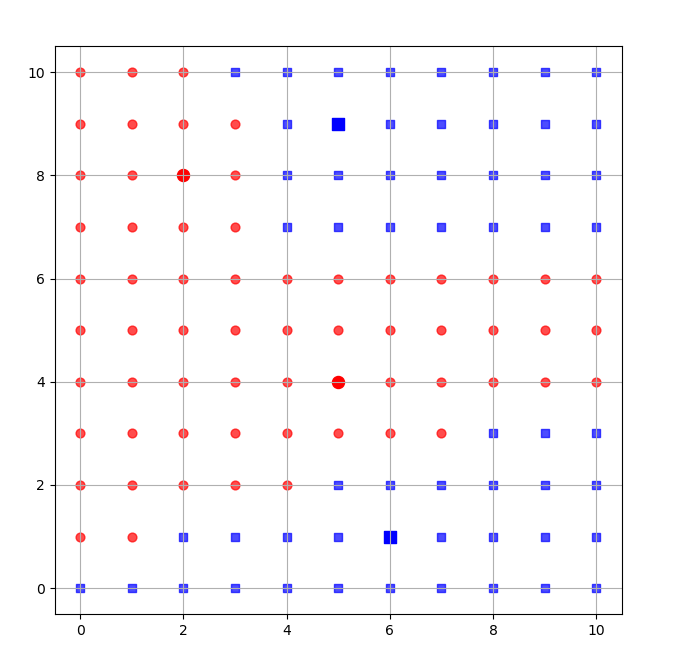
\includegraphics[scale=\myscale,scale=0.25]{ecran-voisins-5}
	\end{center}

	Voici un autre exemple.
	\begin{center}
	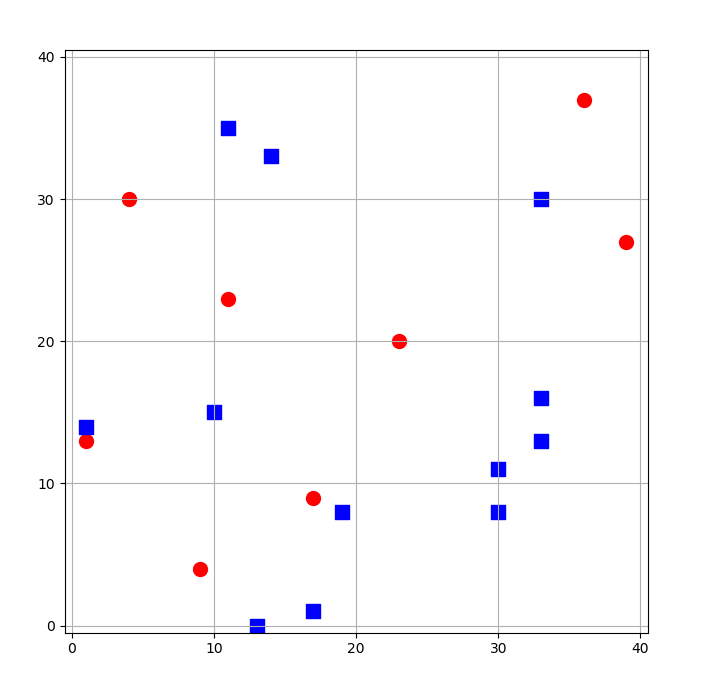
\includegraphics[scale=\myscale,scale=0.25]{ecran-voisins-6} \quad
	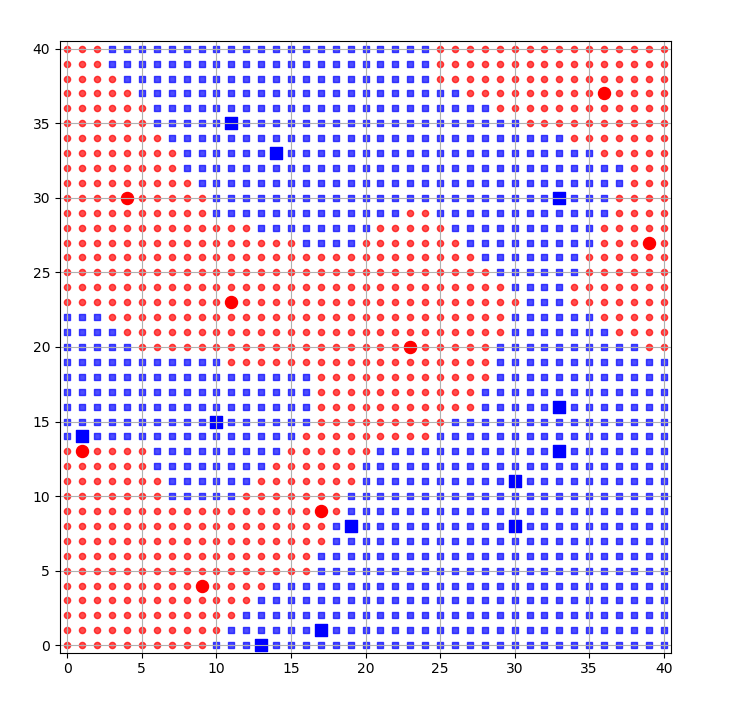
\includegraphics[scale=\myscale,scale=0.25]{ecran-voisins-7}
	\end{center}	
	
	\item \textbf{Les $k$ voisins proches.}
	\begin{enumerate}
		\item Programme une fonction \ci{les_voisins_proches(P,cpoints,k)}
		qui renvoie les $k$ voisins les plus proches du point $P$.
		\begin{itemize}
			\item $P=(x_0,y_0)$ est un point,
			\item \ci{cpoints} est la liste des cpoints $(x,y,c)$ initiaux,
			\item $k\ge1$ est un entier,
			\item la fonction renvoie une liste de $k$ cpoints.
		\end{itemize}  
		 
		\item Programme une fonction \ci{couleur_majoritaire(cpoints)} qui renvoie la couleur majoritaire ($0$ ou $1$) d'une liste de cpoints.
		
		\item Programme une fonction \ci{colorier_par_les_voisins_proches(cpoints,k)} 
		qui à partir d'une liste de points colorés initiaux, colorie tous les autres points : chaque point prend la couleur majoritaire des $k$ voisins les plus proches ($k=1$ correspond au voisin le plus proche).
		
	Ci-dessous à gauche les points colorés initiaux et à droite des coloriages pour différentes valeurs de $k$ ($k=1,2,3$). 
\begin{center}
	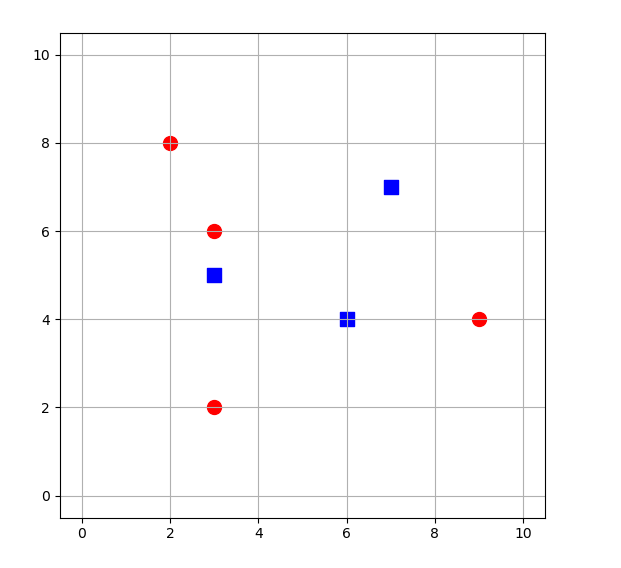
\includegraphics[scale=\myscale,scale=0.17]{ecran-voisins-8a} 
	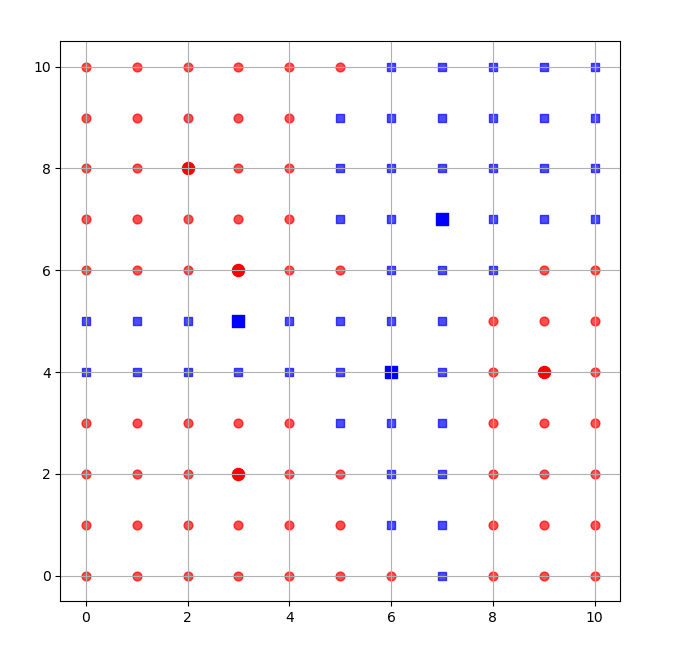
\includegraphics[scale=\myscale,scale=0.146]{ecran-voisins-8b} 
	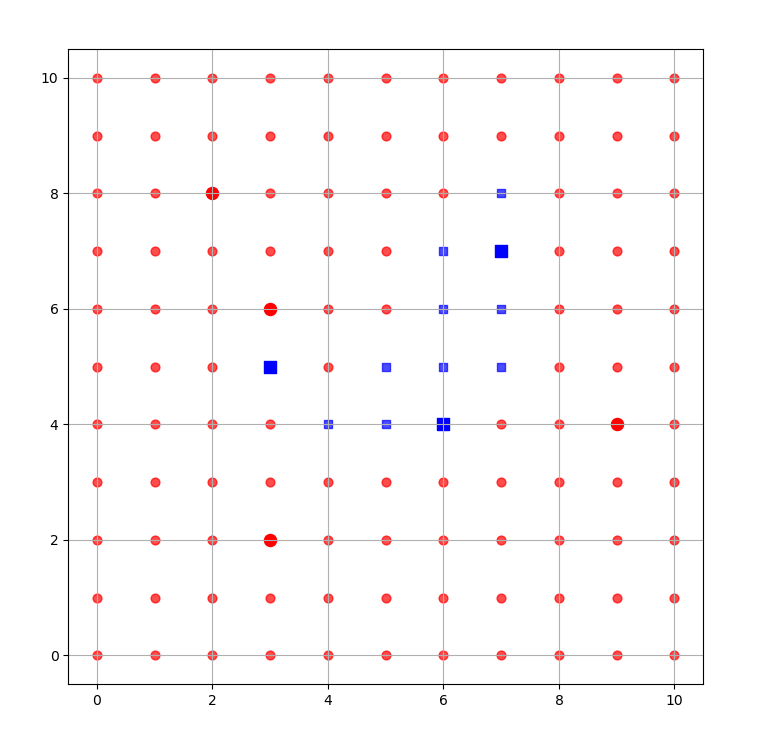
\includegraphics[scale=\myscale,scale=0.13]{ecran-voisins-8c} 
	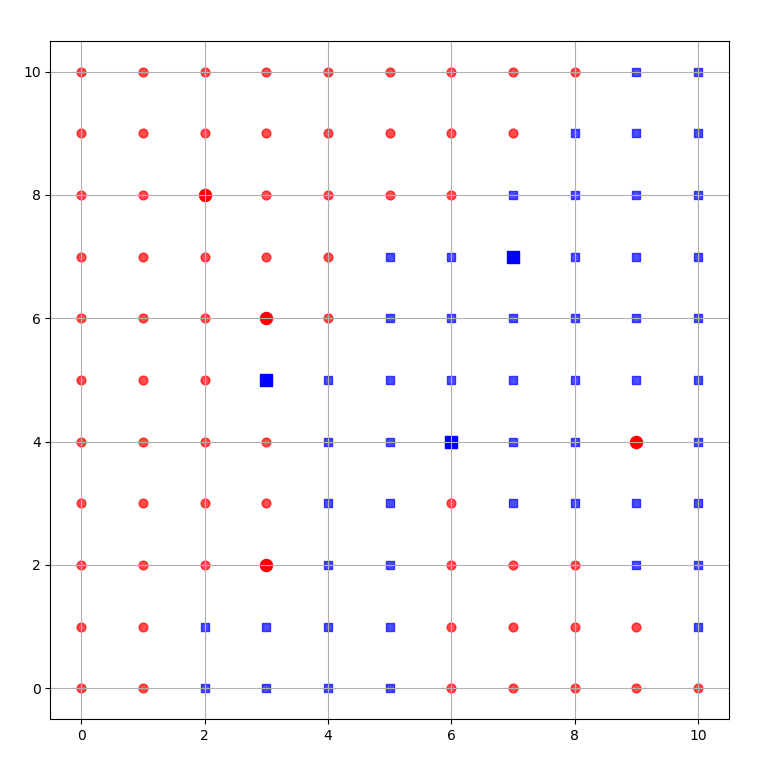
\includegraphics[scale=\myscale,scale=0.128]{ecran-voisins-8d}	
\end{center}

Et voici un exemple de taille plus grande avec $k=3,5,7$.
\begin{center}
	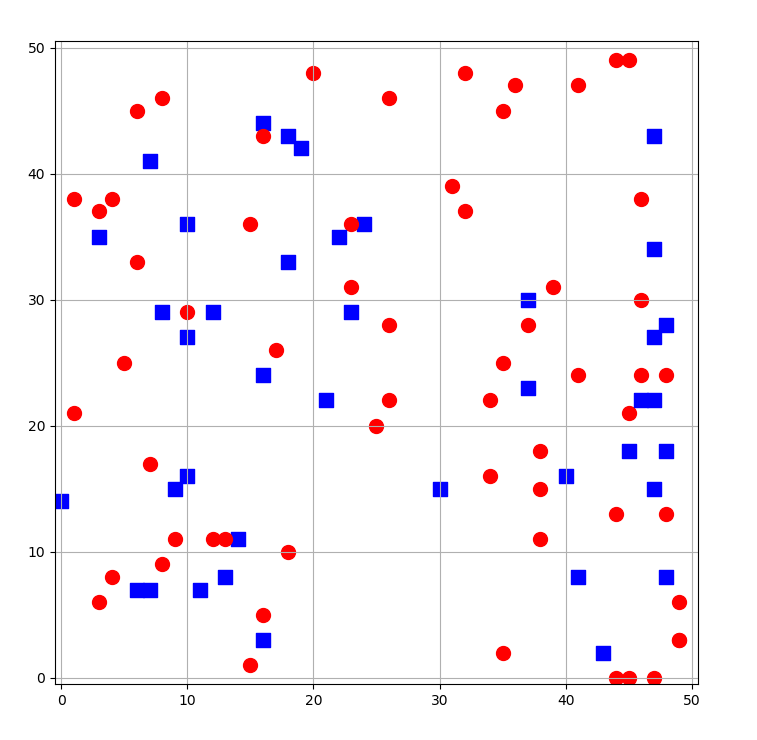
\includegraphics[scale=\myscale,scale=0.133]{ecran-voisins-9a}
	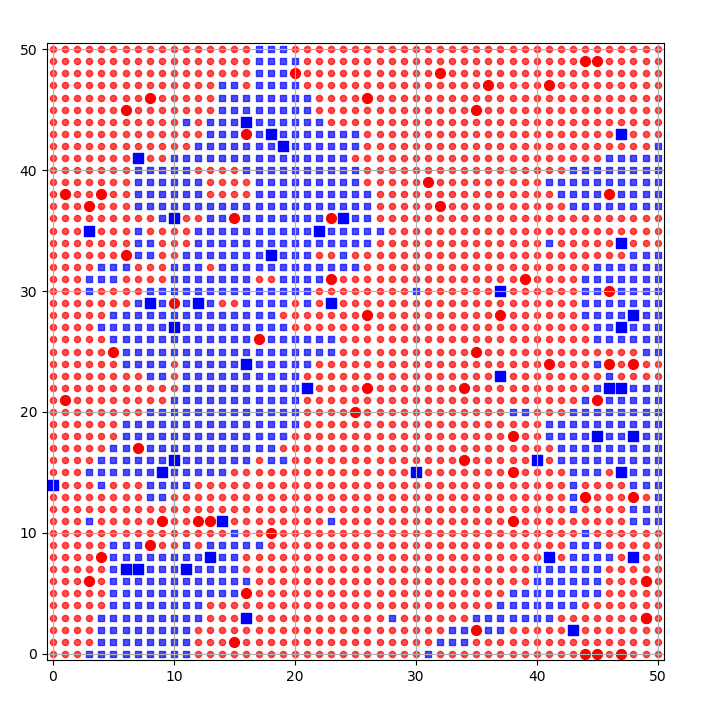
\includegraphics[scale=\myscale,scale=0.137]{ecran-voisins-9b}
	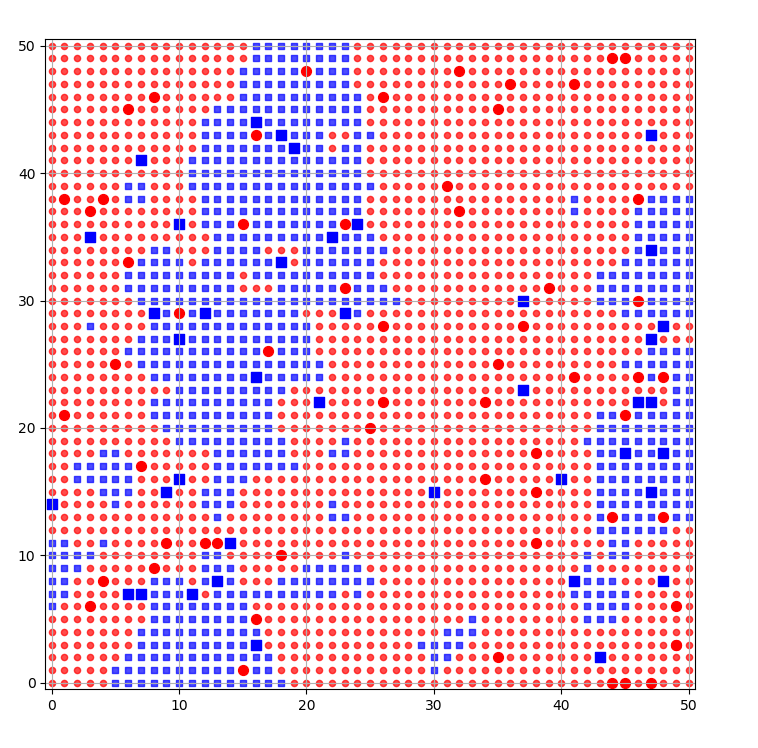
\includegraphics[scale=\myscale,scale=0.133]{ecran-voisins-9c}
	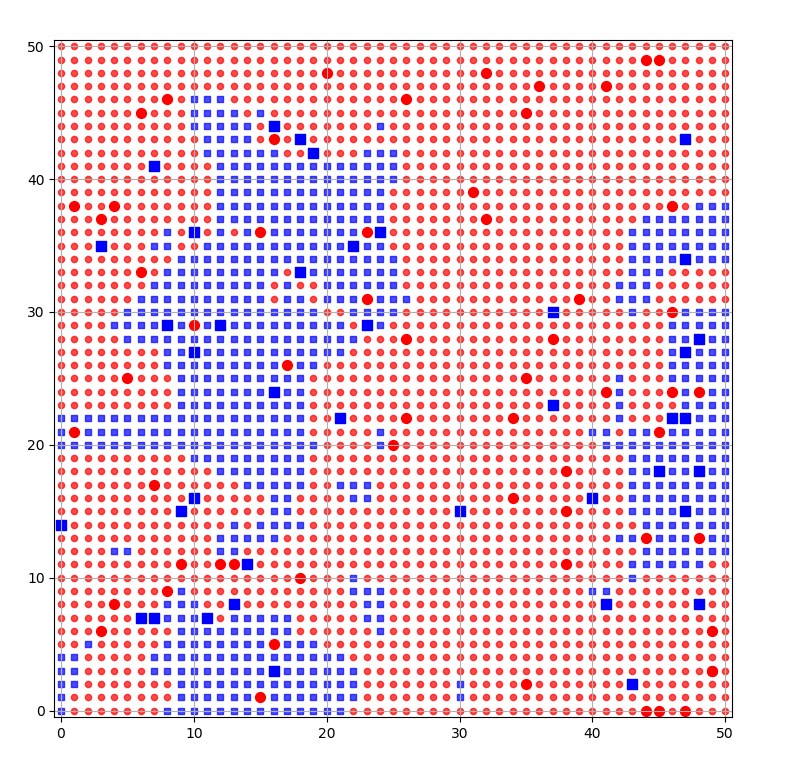
\includegraphics[scale=\myscale,scale=0.13]{ecran-voisins-9d}	
\end{center}		 
		
		
	\end{enumerate}
		
\end{enumerate}
	
\end{activite}


%%%%%%%%%%%%%%%%%%%%%%%%%%%%%%%%%%%%%%%%%%%%%%%%%%%%%%%%%%%%%%%%
%%%%%%%%%%%%%%%%%%%%%%%%%%%%%%%%%%%%%%%%%%%%%%%%%%%%%%%%%%%%%%%%

\begin{cours}[Expression correctement parenthésée]
Voici des exemples d'expressions bien et mal parenthésées :
\begin{itemize}
	\item $2 + (3 + b) \times (5 + (a - 4))$ est correctement parenthésée ;
	\item $(a+ 8) \times 3 ) + 4$ est mal parenthésée : il y a une parenthèse fermante \og{}$)$\fg{}  seule ;
	\item $(b + 8 / 5)) + (4$ est mal parenthésée : il y a autant de parenthèses ouvrantes 
	\og{}$($\fg{} que de parenthèses fermantes \og{}$)$\fg{} mais elles sont mal positionnées.
\end{itemize}


Dans le chapitre \og{}Calculatrice polonaise – Piles\fg{} du premier tome, nous avions étudié un algorithme qui vérifie si une expression a ses parenthèses bien agencées. 
Cette méthode résout complètement le problème mais nécessite beaucoup de mémoire. En effet la taille de la pile peut être de l'ordre de grandeur de la longueur de l'expression, ce qui pose des problèmes pour des expressions ayant des millions de caractères. Par contre, avec la méthode de l'activité suivante tu ne stockes que les valeurs de deux entiers ($h$ et $S$), l'inconvénient c'est que la réponse renvoyée est probablement vraie,
mais ce n'est pas une certitude. 
Cette méthode permet aussi de vérifier si un fichier (par exemple un fichier \og{}xml\fg{}) a un balisage correct.
\end{cours}


%%%%%%%%%%%%%%%%%%%%%%%%%%%%%%%%%%%%%%%%%%%%%%%%%%%%%%%%%%%%%%%%
% Activité ? - Parenthèses correctes ?
%%%%%%%%%%%%%%%%%%%%%%%%%%%%%%%%%%%%%%%%%%%%%%%%%%%%%%%%%%%%%%%%

% D'après Claire Mathieu - cours au Collège de France

\begin{activite}[Parenthèses correctes ?]
	
\objectifs{Objectifs : tester si une expression a ses parenthèses et ses crochets bien agencés.}


\textbf{Partie A. Parenthèses seules.}

On considère une expression avec des parenthèses (tous les autres caractères sont ignorés). 
On associe une hauteur $h$ en lisant l'expression de gauche à droite :
\begin{itemize}
	\item au départ $h=0$,
	\item \emph{avant} une parenthèse ouvrante \ci{"("} on augmente $h$ de $1$,
	\item \emph{après} une parenthèse fermante \ci{")"} on diminue $h$ de $1$.
\end{itemize}

Voici un exemple avec l'expression \og{}$n=(2\times(3+4)+5)-6$\fg{}.
\myfigure{0.4}{
	\tikzinput{fig_parentheses_1a}
}


On fixe un nombre premier $p$ (par exemple $p=11$ ou $p=101$) et on pose $a=2$.
\`A chaque parenthèse on associe un entier modulo $p$ :
$$ \text{\ci{"("}} \mapsto 2^h \pmod{p} \quad \text{ et }\quad \text{\ci{")"}} \mapsto -2^h \pmod{p},$$
à tous les autres caractères on associe $0$. Ensuite on calcule la somme $S$ de tous ces termes.

\myfigure{0.4}{
	\tikzinput{fig_parentheses_1b}
}

\begin{itemize}
 \item Si l'expression est bien parenthésée alors $S=0$.
 \item Si à un moment $h<0$ ou si à la fin $S \neq 0$ alors l'expression est mal parenthésée.
\end{itemize}

\bigskip

Programme cette méthode en une fonction \ci{test_parentheses(expression)} qui renvoie
\og{}Vrai\fg{} si la somme de contrôle vaut $0$ et \og{}Faux\fg{} sinon.


Voici un exemple d'une expression mal parenthésée : \og{}$x(x)x(x(x)x$\fg{} (ici $x$ désigne n'importe quelle suite de caractères autre que des parenthèses), le problème est bien détecté car la somme $S=2$ n'est pas nulle.

\myfigure{0.4}{
	\tikzinput{fig_parentheses_2}
}

\bigskip

\textbf{Partie B. Parenthèses et crochets.}

On va améliorer cette fonction pour tester une expression avec des parenthèses et des crochets.
Voici une expression cohérente \og{}$[(a+b)\times(a-b)]$\fg{} ; voici des expressions non correctes \og{}$[a+b)$\fg{} ou \og{}$(a\times[b+c)-d]$\fg{}.


On considère une expression avec des parenthèses et des crochets (tous les autres caractères sont ignorés). On associe une hauteur $h$ en lisant l'expression de gauche à droite, au départ 
$h=0$, on augmente $h$ de $1$ \emph{avant} une parenthèse ou un crochet ouvrant, \ci{"("} ou \ci{"["}, on diminue $h$ de $1$ \emph{après} une parenthèse ou un crochet fermant, \ci{")"} ou  \ci{"]"}.

On fixe un nombre premier $p$ assez grand (par exemple $p=11$ ou $p=101$) et on pose $a=2$ et $b=3$.
\`A chaque parenthèse on associe comme auparavant un entier modulo $p$ :
$$ \text{\ci{"("}} \mapsto 2^h \pmod{p} \quad \text{ et }\quad \text{\ci{")"}} \mapsto -2^h \pmod{p}.$$
\`A chaque crochet on associe aussi un entier modulo $p$ :
$$ \text{\ci{"["}} \mapsto 3^h \pmod{p} \quad \text{ et }\quad \text{\ci{"]"}} \mapsto -3^h \pmod{p}.$$
\`A tous les autres caractères on associe $0$.
Ensuite on calcule la somme $S$ de tous ces termes.



\begin{itemize}
	\item Si l'expression est bien parenthésée et crochetée alors $S=0$.
	\item Si à un moment $h<0$ ou si à la fin $S \neq 0$ alors l'expression est mal parenthésée ou mal crochetée.
	\item Il peut y avoir des cas exceptionnels où $S=0$ et cependant l'expression est mal parenthésée/crochetée.
\end{itemize}

Programme une fonction \ci{test_crochets_parentheses(expression)} qui renvoie
\og{}Vrai\fg{} si la somme de contrôle vaut $0$ et \og{}Faux\fg{} sinon.


Voici deux exemples.
\myfigure{0.4}{
	\tikzinput{fig_parentheses_3}
}

\myfigure{0.4}{
	\tikzinput{fig_parentheses_4}
}

Teste ta fonction sur les deux exemples suivants :
\mycenterline{\ci{"[([[]][[[[(()[(()([((())[[]])]))])]]]])]"}}
\mycenterline{\ci{"[[[()](()[((([[]])()(([[[]][()]]])))])]]"}}


On a une certitude uniquement dans le cas où $S\neq0$ (l'expression est alors mal parenthésée/crochetée),
dans le cas $S=0$ on a seulement une forte probabilité que l'expression soit bien parenthésée/crochetée.
Voici des exemples de situations non détectées. Par exemple \ci{"[)(]"} (mais si on regarde juste les parenthèses on voit que l'expression n'est déjà pas correcte). Il faut donc au préalable vérifier que les parenthèses seules sont bien positionnées, et aussi que les crochets seuls sont bien positionnés. 
Autre soucis possible avec \ci{"(["} et $p=11$ alors on trouve une somme $S=2^1+3^2=11$ donc 
$S=0 \pmod{11}$ et pourtant l'expression est mal parenthésée/crochetée.
Par contre avec $p=7$, on trouve $S=4 \pmod{7}$, donc cela prouve que l'expression est mal parenthésée/crochetée.

\emph{Note.} Cet algorithme peut être programmé en temps réel, c'est-à-dire que l'on peut commencer les calculs dès la lecture du premier caractère et les terminer juste après le dernier.
\end{activite}




%%%%%%%%%%%%%%%%%%%%%%%%%%%%%%%%%%%%%%%%%%%%%%%%%%%%%%%%%%%%%%%%
%%%%%%%%%%%%%%%%%%%%%%%%%%%%%%%%%%%%%%%%%%%%%%%%%%%%%%%%%%%%%%%%

\begin{cours}[Isobarycentre]

\index{barycentre}

On considère $n$ points du plan $P_1$, $P_2$,\ldots,$P_n$.
On cherche un point \og{}le plus au milieu possible\fg{} de tous ces points. On appelle ce point \defi{l'isobarycentre} des $\{P_i\}$ et on le note $G$.

\myfigure{1}{
	\tikzinput{fig-barycentres-2}
}

\textbf{Cas de deux points.} Si $n=2$ alors
	$G$ est simplement le milieu du segment $[P_1,P_2]$.
	
\textbf{Cas de trois points.} Si $n=3$ alors
$G$ est le centre de gravité du triangle défini par les trois points. C'est donc l'intersection des médianes.	
	
\myfigure{0.7}{
	\tikzinput{fig-barycentres-1}
}	

	

	
\textbf{Formule.}
Pour $n$ quelconque, voici la formule pour calculer les coordonnées $(x_G,y_G)$ de l'isobarycentre $G$ en fonction des coordonnées $(x_i,y_i)$ des $P_i$ ($i=1,\ldots,n$) :
\mybox{$\displaystyle x_G = \frac{x_1+x_2+\cdots+x_n}{n} \qquad \text{ et } \qquad y_G = \frac{y_1+y_2+\cdots+y_n}{n}$}




Cela signifie que l'abscisse de $G$ est simplement la moyenne des abscisses des $P_i$ et l'ordonnée de $G$ est la moyenne des ordonnées des $P_i$.
Pour $n=2$ on retrouve les coordonnées du milieu $\left(\frac{x_1+x_2}{2}, \frac{y_1+y_2}{2}\right)$. Et pour $n=3$ cela donne 
$$(x_G,y_G) = \left(\frac{x_1+x_2+x_3}{3},\frac{y_1+y_2+y_3}{3}\right).$$

\end{cours}


%%%%%%%%%%%%%%%%%%%%%%%%%%%%%%%%%%%%%%%%%%%%%%%%%%%%%%%%%%%%%%%%
% Activité 3 - Barycentres
%%%%%%%%%%%%%%%%%%%%%%%%%%%%%%%%%%%%%%%%%%%%%%%%%%%%%%%%%%%%%%%%

\begin{activite}[Barycentres]
	
\objectifs{Objectifs : rassembler des points en groupes.}

\emph{Note.} Certaines fonctions sont très proches de la première activité sur les $k$ voisins.

\begin{enumerate}
	\item \textbf{Afficher des points.}
	
	Programme d'abord une fonction \ci{afficher_points(points,couleurs)}
	qui affiche une liste de points $(x,y)$ en fonction d'une liste de couleurs (une couleur par point).
	
	Par exemple avec \ci{points = [(20,20),(60,40),(40,80),(70,70)]} et \ci{couleurs = [0,1,2,0]}
	alors \ci{afficher_points(points,couleurs)} affiche le graphique ci-dessous.
	
	\begin{center}
	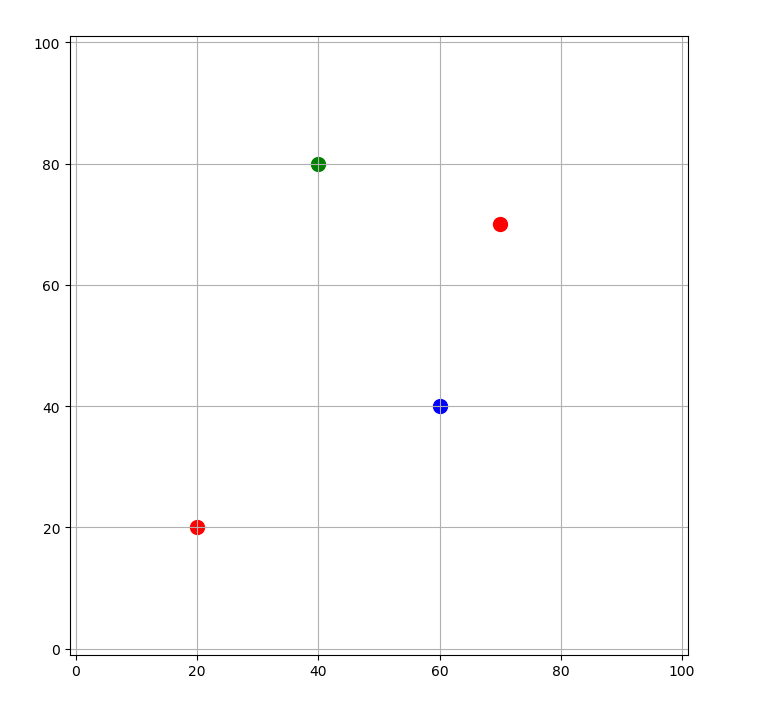
\includegraphics[scale=\myscale,scale=0.17]{ecran-barycentres-1} 
	\end{center}
	
	\emph{Indications.} 
	\begin{itemize}
		\item Tu peux définir des constantes $x_{\min}$, $x_{\max}$, $y_{\min}$, $y_{\max}$
		pour définir une fenêtre de visualisation. On prendra par défaut $[0,100]\times[0,100]$.
		
		\item Pour les couleurs, $0$ peut être pour le rouge, $1$ pour le bleu\ldots
	\end{itemize}

	\item \textbf{Générer des points.}
	
	On veut générer des groupes aléatoires de points, comme ci-dessous à gauche avec trois groupes de points. Chaque groupe est généré au hasard autour d'un centre, avec un paramètre de dispersion qui fait que les points s'éloignent plus ou moins du centre (voir les trois figures de droite : un seul groupe de points mais avec des paramètres de dispersion différents).
	
	\begin{center}
		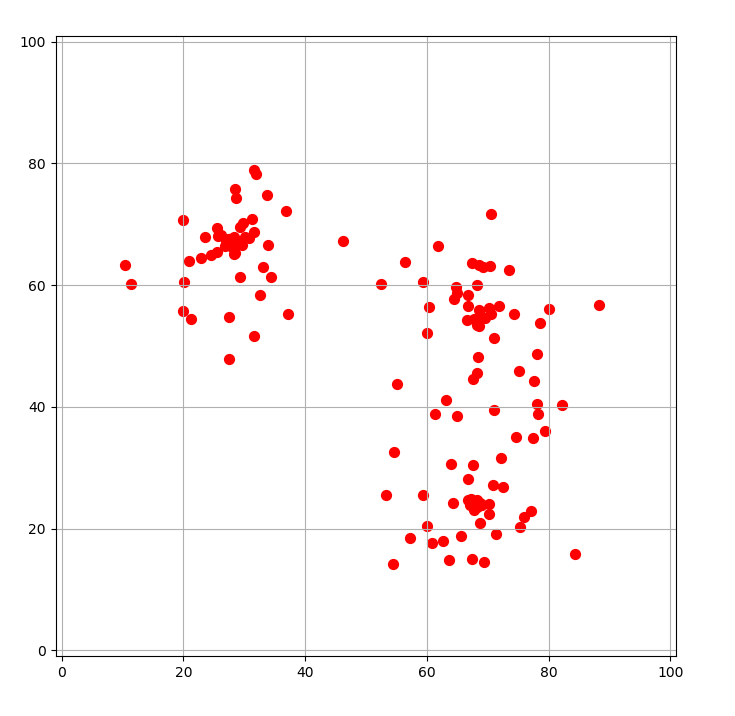
\includegraphics[scale=\myscale,height=3.5cm]{ecran-barycentres-2}
		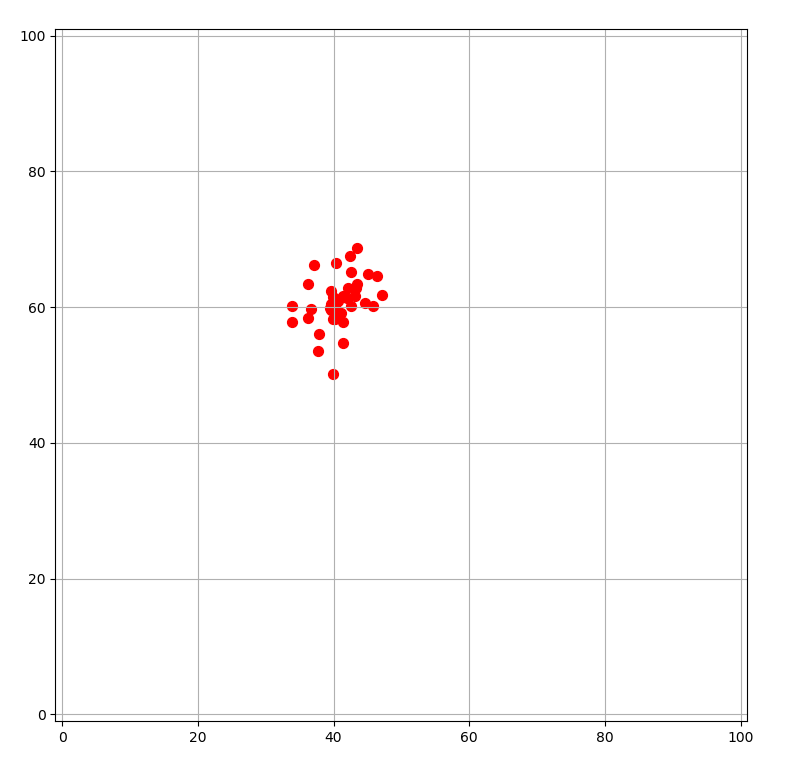
\includegraphics[scale=\myscale,height=3.5cm]{ecran-barycentres-3a}
		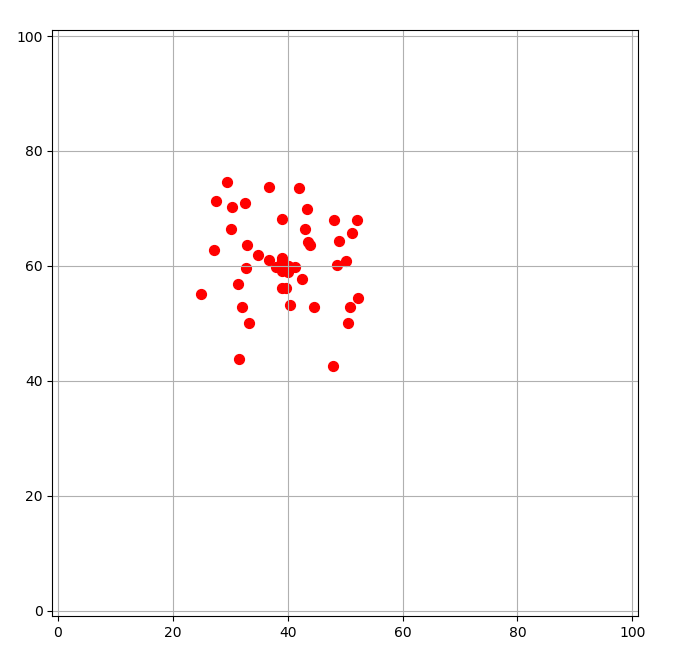
\includegraphics[scale=\myscale,height=3.5cm]{ecran-barycentres-3b}
		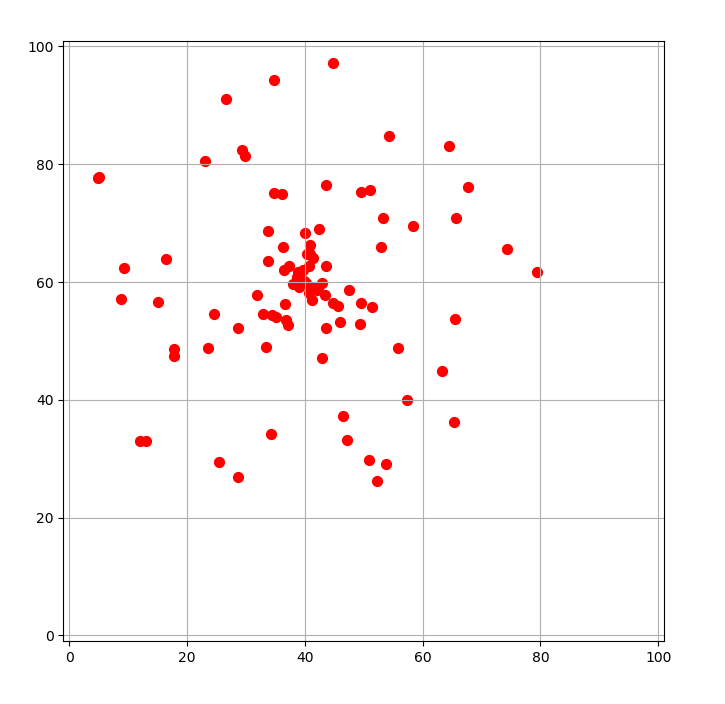
\includegraphics[scale=\myscale,height=3.5cm]{ecran-barycentres-3c}
	\end{center}
	
	Voici comment programmer une fonction \ci{generer_points(k,n,d)}
	qui affiche $k$ groupes, de $n$ points chacun, selon une dispersion $d$.
	
	Répéter $k$ fois :
	\begin{itemize}
		\item Choisir un centre $(x_c,y_c)$ au hasard dans la fenêtre (c'est mieux s'il n'est pas trop près des bords).
		
		\item Pour ce centre, répéter $n$ fois :
		\begin{itemize}
			\item Choisir un angle $\theta$ au hasard entre $0$ et $2\pi$.
			\item Choisir un rayon $r$ au hasard selon la formule $r = d \rho^2$ où $\rho$ est un réel tiré au hasard entre $0$ et $1$.
			\item Ajoute le point $(x,y)$ à la liste des points, où :
			$$x = x_c + r \cos \theta \qquad \text{ et } \qquad y = y_c + r \sin \theta$$
			(vérifie que $(x,y)$ est bien dans la fenêtre voulue).
		\end{itemize}
	\end{itemize}
	
	\emph{Indications.} La fonction \ci{random()} (sans argument) du module \ci{random} renvoie à chaque appel un nombre flottant aléatoire $x$ de $[0,1[$.
	Pour obtenir à partir de $x$ un nombre aléatoire $y$ entre $a$ et $b$, on peut utiliser la formule :
	$$y = a + (b-a)x.$$
	
	\item \textbf{Calcul du barycentre.}	
	
	Programme une fonction \ci{calcul_barycentre(points)} qui calcule l'isobarycentre $(x_G,y_G)$ d'une liste de points $\{(x_i,y_i)\}$. On rappelle la formule :
	$$x_G = \frac{x_1+x_2+\cdots+x_n}{n} \quad \text{ et } \quad y_G = \frac{y_1+y_2+\cdots+y_n}{n}.$$
	
	\emph{Exemple.} Avec les points $(20,60)$, $(40,20)$, $(60,80)$\couleurnb{ (en rouge)}{} la fonction calcule les coordonnées du barycentre $(x_G,y_G) = (40, 53.33\ldots)$\couleurnb{ (en bleu)}{}.
	
		\begin{center}
		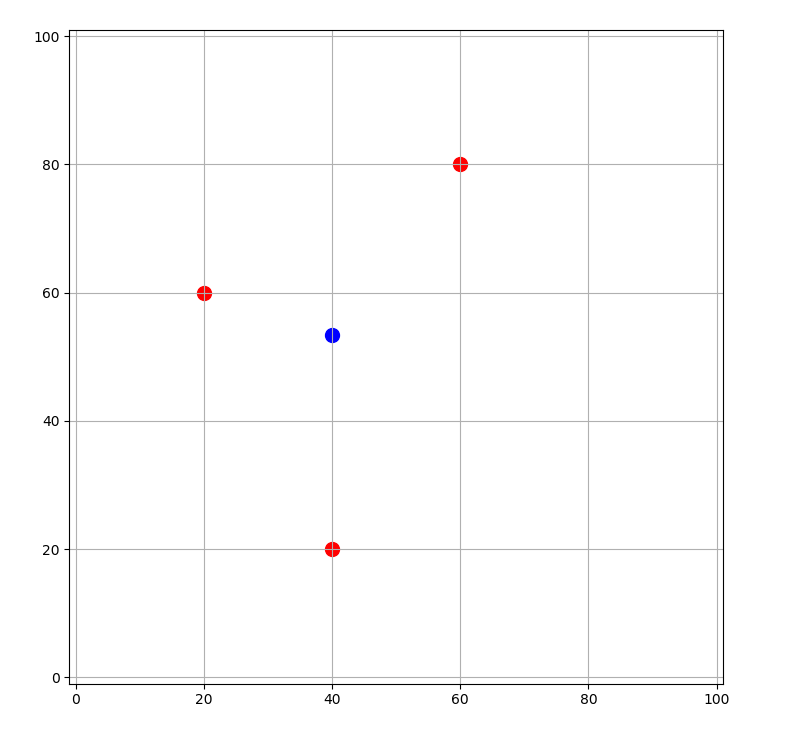
\includegraphics[scale=\myscale,scale=0.2]{ecran-barycentres-4}
	\end{center}
	
	\item \textbf{Barycentre le plus proche.}
	
	Dans cette question on se donne une liste de barycentres (on verra plus tard comment on les obtient)
	et une liste de points. Pour chaque point on va trouver quel est le barycentre le plus proche.
	
	\begin{enumerate}
		\item Programme une fonction \ci{distance(P,Q)} qui calcule la distance entre $P = (x_1,y_1)$ et $Q=(x_2,y_2)$ :
		$$d = \sqrt{(x_1-x_2)^2 + (y_1-y_2)^2}.$$
		
		\item Programme une fonction \ci{barycentre_proche(P,barycentres)}
		qui à partir d'un point $P=(x_0,y_0)$ renvoie le rang du point le plus proche dans la liste \ci{barycentres} donnée.
		
		Par exemple, si nous avons la liste \ci{barycentres = [(80,40),(20,80),(60,60)]}\couleurnb{ (en rouge)}{}
		et le point $P=(40,40)$\couleurnb{ (en noir)}{}, alors le barycentre le plus proche de $P$ est $G_2=(60,60)$ qui est de rang $2$ dans la liste des barycentres. Donc la fonction \ci{barycentre_proche(P,barycentres)} renvoie ici $2$.
		
		\begin{center}
		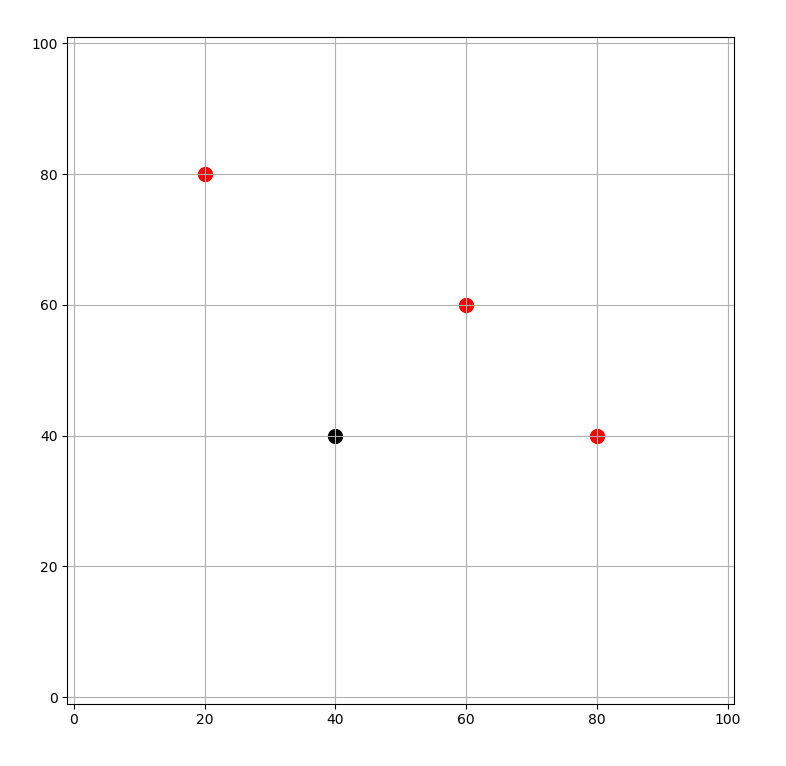
\includegraphics[scale=\myscale,scale=0.2]{ecran-barycentres-5}
		\end{center}

	
		\item \textbf{Coloriage suivant le barycentre le plus proche.}			
		La fonction précédente renvoie le rang du barycentre le plus proche et on considère ce rang comme la couleur (le barycentre $G_0$ en tête de liste est de couleur $0$ donc rouge, le barycentre $G_1$ est de couleur $1$ donc bleu\ldots).
		
		Déduis-en une fonction \ci{couleurs_barycentres_proches(points,barycentres)}
		qui à partir d'une liste de points renvoie la liste des couleurs attribuées à chaque point (selon le rang du barycentre le plus proche, c'est-à-dire la couleur).
		
		\emph{Exemple.} Reprenons nos barycentres \ci{barycentres = [(80,40), (20,80), (60,60)]} avec chacun une couleur donnée par son rang : $G_0=(80,40)$ est de couleur $0$ (rouge), $G_1=(20,80)$ est de couleur $1$ (bleu),
		$G_2=(60,60)$ est de couleur $2$ (vert). Fixons aussi une liste de points \ci{points = [(40,40),(20,40),(80,70),(50,10)]} pour l'instant sans couleur (\couleurnb{en noir sur la }figure de gauche ci-dessous). Alors la fonction \ci{couleurs_barycentres_proches()} renvoie la liste \ci{[2, 1, 2, 0]}. Cela signifie que le point $P_0=(40,40)$ doit être colorié par la couleur $2$ car le plus proche barycentre est $G_2$, le point $P_1=(20,40)$ doit être colorié par la couleur $1$ car le plus proche barycentre est $G_1$\ldots{} Cela permet de colorier les quatre points (figure de droite).
		
		\begin{center}
		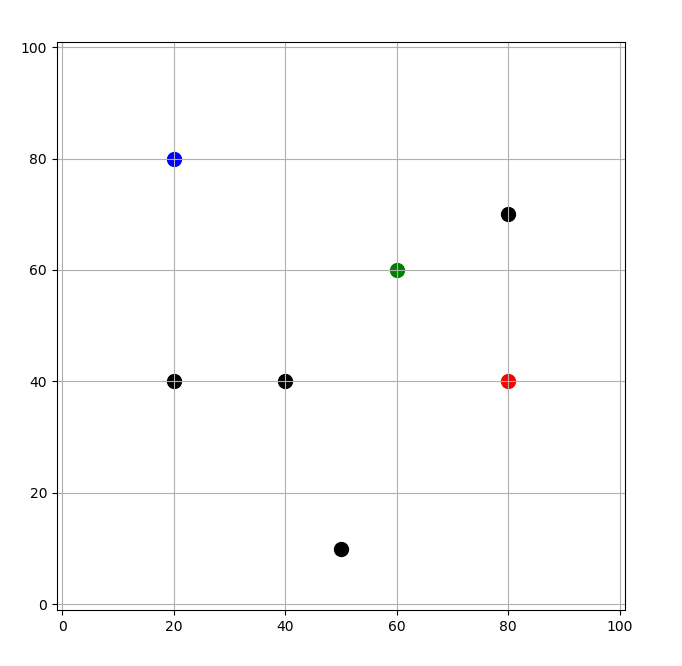
\includegraphics[scale=\myscale,scale=0.26]{ecran-barycentres-6a}\qquad
		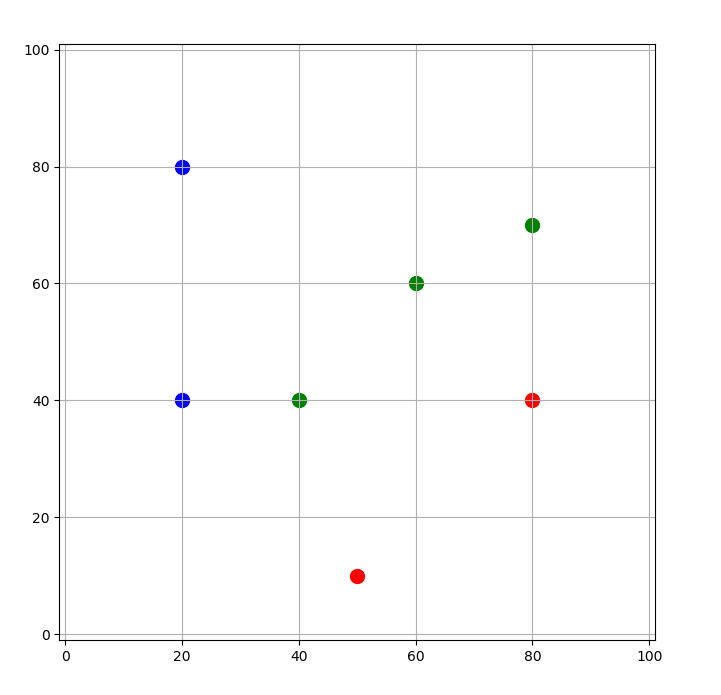
\includegraphics[scale=\myscale,scale=0.25]{ecran-barycentres-6b}
		\end{center}		
		
	\end{enumerate}

	\item \textbf{Recalculer les barycentres.}
	
	\begin{itemize}
	    \item On se donne une liste de points et une liste de barycentres (figure de gauche ci-dessous, pour l'instant cette liste de \og{}barycentres\fg{} est arbitraire).
     	\item On a vu comment attribuer une couleur à chaque point (figure centrale), ainsi les points sont regroupés par couleur. \couleurnb{Les points bleus sont associés au barycentre bleu clair, les points verts sont associés au barycentre vert clair\ldots}{}
     	\item Pour tous les points d'une même couleur, on calcule le barycentre. On se retrouve avec une nouvelle liste de barycentres (figure de droite) (cette fois ce sont de \og{}vrais\fg{} barycentres).
     \end{itemize}
 
	\begin{center}
		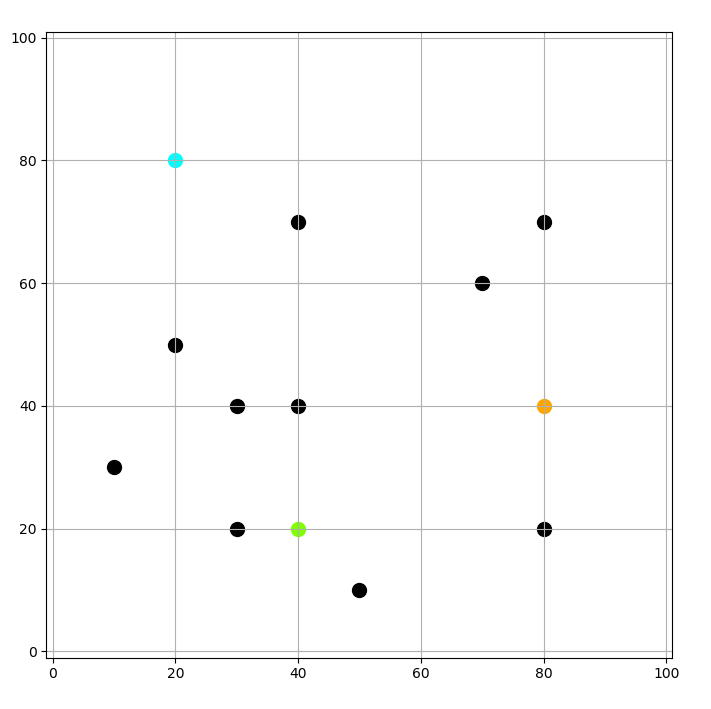
\includegraphics[scale=\myscale,scale=0.173]{ecran-barycentres-7a}\quad
		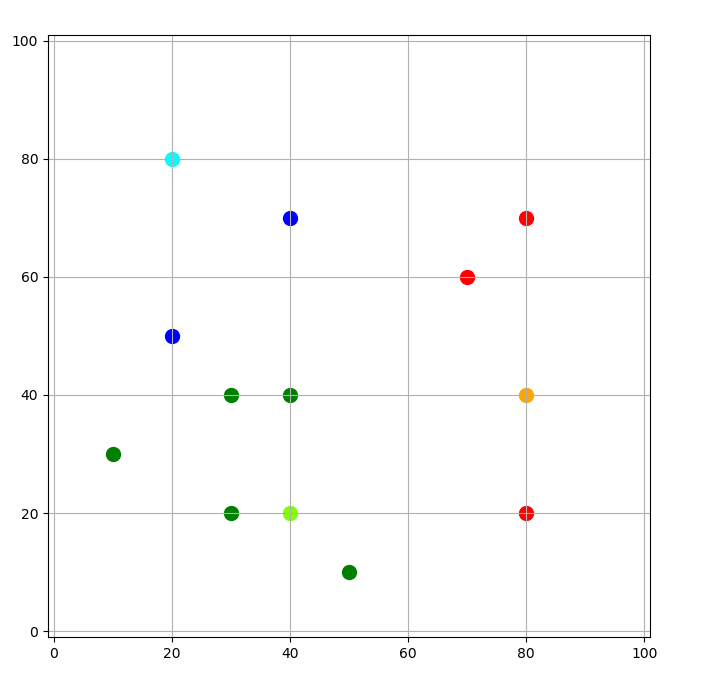
\includegraphics[scale=\myscale,scale=0.18]{ecran-barycentres-7b}\quad
		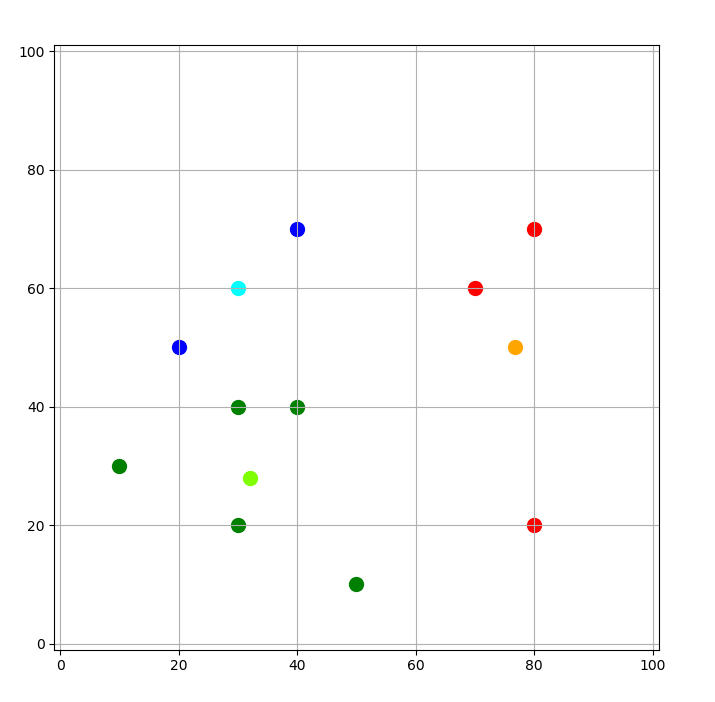
\includegraphics[scale=\myscale,scale=0.18]{ecran-barycentres-7c}
	\end{center}
	
	Programme une fonction \ci{recalculer_barycentres(points,barycentres)} qui effectue cette tâche.	
	Sur l'exemple graphique ci-dessus les barycentres de départs sont $[(80,40),(20,80),(40,20)]$ (figure de gauche), la fonction \ci{recalculer_barycentres()} renvoie les coordonnées des nouveaux barycentres : $[(76.66\ldots, 50), (30, 60), (32, 28)]$.
	 
	\emph{Indications.} Si un barycentre n'est associé à aucun point on le conserve inchangé.
	
	\item\textbf{Itérer les barycentres.}
	
	Voici comment regrouper des points en les coloriant par groupe. Sur la figure de gauche on a tiré des points (presque) au hasard (on devine à peine $3$ groupes). Sur la figure de droite, l'algorithme a séparé les points en $3$ groupes pertinents (avec en noir les $3$ barycentres que l'on va déterminer).
	
	\begin{center}
		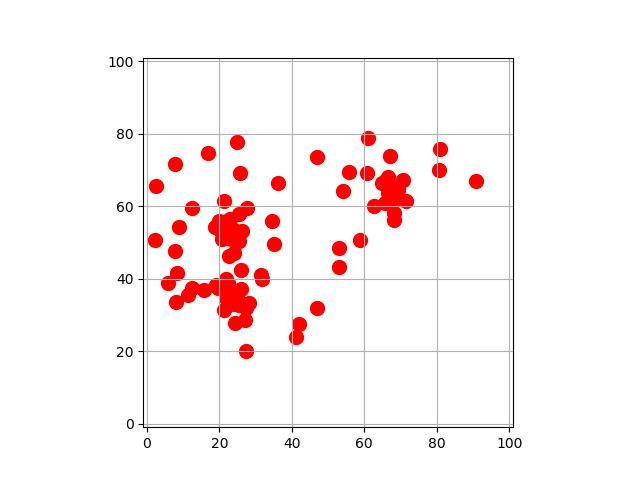
\includegraphics[scale=\myscale,scale=0.5]{ecran_barycentres_exemple_01}\quad
		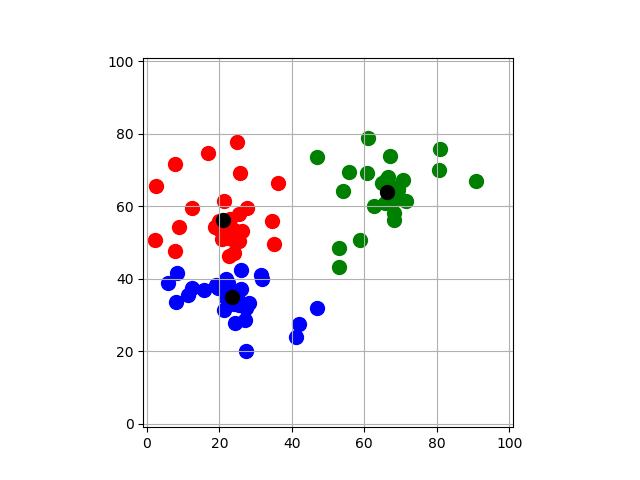
\includegraphics[scale=\myscale,scale=0.5]{ecran_barycentres_exemple_10}
	\end{center}	
	
	Voici les étapes graphiques de l'algorithme. Sur la figure de gauche ci-dessous, on part de trois points (en noir) qui jouent le rôle de barycentres initiaux (on les choisit au hasard ou bien trois points assez écartés de la fenêtre).
	On colorie les autres points selon le barycentre le plus proche. \'Etape suivante (figure du milieu) on calcule le nouveau barycentre pour les points rouges, le nouveau barycentre  pour les points bleus\ldots{} mais alors on doit aussi recalculer la couleur de tous les autres points (puisque les coordonnées des barycentres ont changé). On itère le processus (autres figures) jusqu'à ce que les couleurs des points ne changent plus.
	 

	
	\begin{center}
	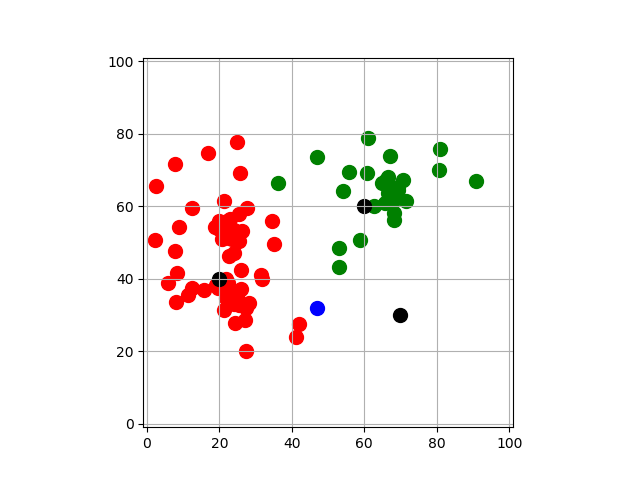
\includegraphics[scale=\myscale,scale=0.32]{ecran_barycentres_exemple_02}
	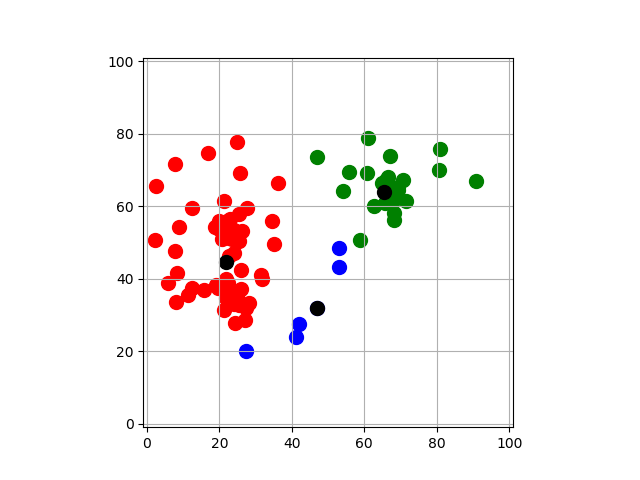
\includegraphics[scale=\myscale,scale=0.32]{ecran_barycentres_exemple_03}
	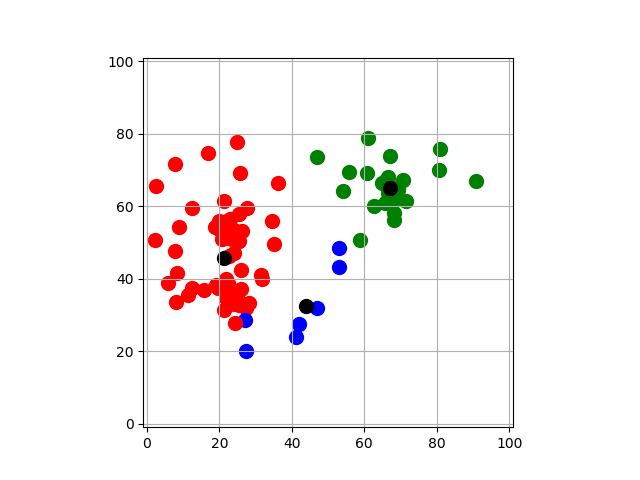
\includegraphics[scale=\myscale,scale=0.32]{ecran_barycentres_exemple_04}
	\end{center}	
	\begin{center}
	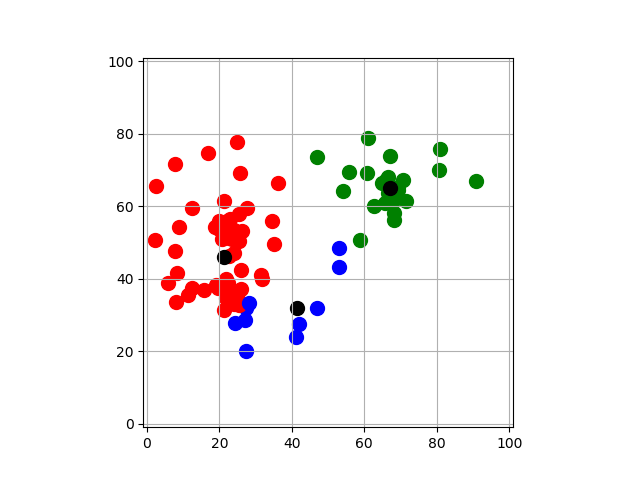
\includegraphics[scale=\myscale,scale=0.32]{ecran_barycentres_exemple_05}
	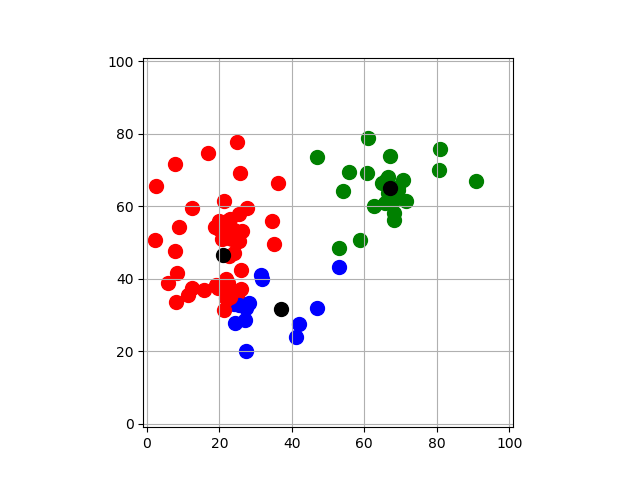
\includegraphics[scale=\myscale,scale=0.32]{ecran_barycentres_exemple_06}
	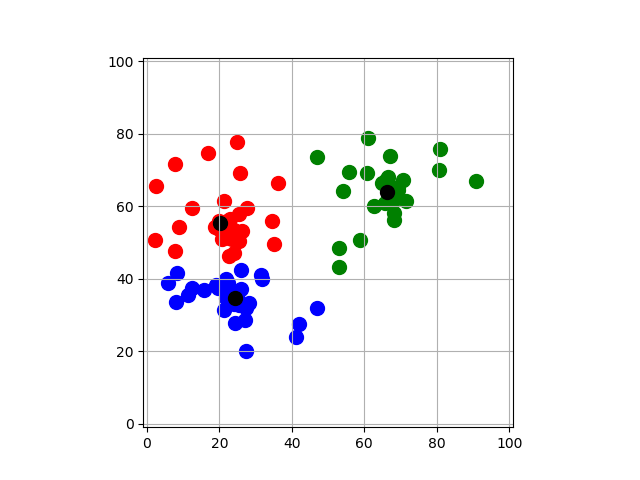
\includegraphics[scale=\myscale,scale=0.32]{ecran_barycentres_exemple_09}
	\end{center}	

	Programme une fonction \ci{iterer_barycentres(points,barycentres_init)} qui effectue cette tâche.
	
	\smallskip
	
	\emph{Indications.}
	\begin{itemize}	
		\item Il s'agit juste, à chaque étape, d'utiliser la fonction \ci{recalculer_barycentres()}
		suivie de \ci{couleurs_barycentres_proches()} avec les nouvelles coordonnées des barycentres.
		
		\item On itère ces étapes jusqu'à ce que la liste des couleurs se stabilise (ou bien après un nombre fixé d'étapes).
		
		\item Pour remplacer la liste des anciens barycentres par la liste des nouveaux, utilise :		
		\mycenterline{\ci{barycentres = list(nouv_barycentres)}}
	\end{itemize}
\end{enumerate}

\medskip

On termine par un exemple avec $5$ groupes de points (à gauche les points de départ, au centre les $5$ barycentres initiaux et le premier coloriage, à droite le résultat après plusieurs itérations). Il faut parfois tester différentes configurations des barycentres initiaux pour que cela fonctionne bien.
	\begin{center}
	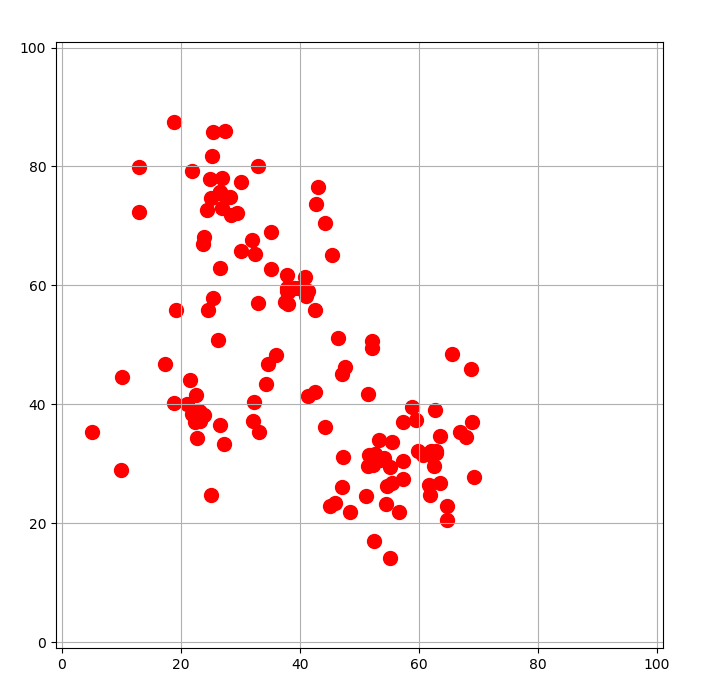
\includegraphics[scale=\myscale,scale=0.21]{ecran_barycentres_exemple_bis_01}\quad
	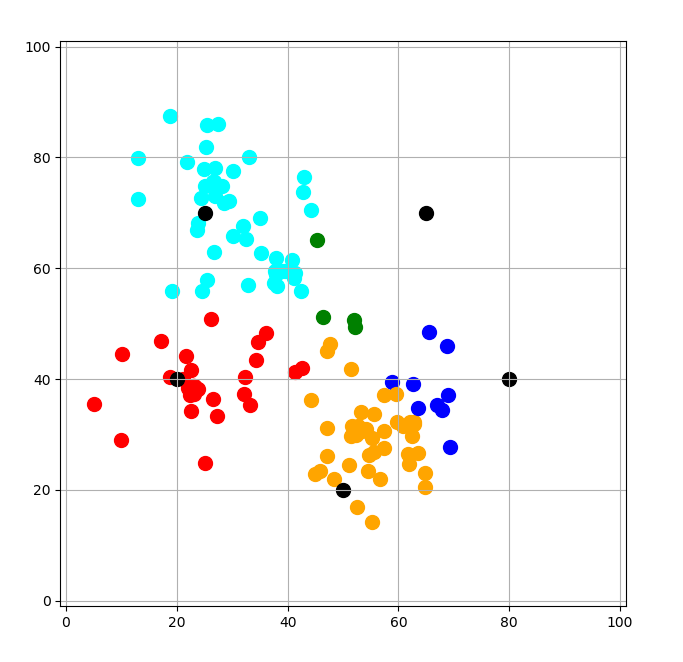
\includegraphics[scale=\myscale,scale=0.22]{ecran_barycentres_exemple_bis_02}\quad
	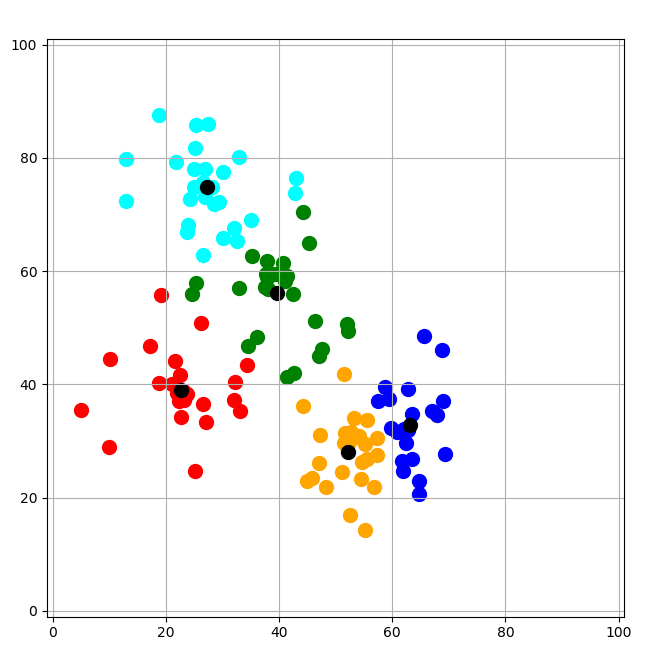
\includegraphics[scale=\myscale,scale=0.22]{ecran_barycentres_exemple_bis_05}
\end{center}

\bigskip



\emph{Note.} 

Il y a une différence fondamentale entre cette activité et l'activité sur les  $k$ voisins. Il s'agit ici d'un \emph{apprentissage non supervisé}, c'est-à-dire qu'on laisse l'algorithme trouver tout seul les groupes. L'activité sur les $k$ voisins est celle d'un \emph{apprentissage supervisé} : certains points sont déjà coloriés rouge ou bleu et servent de référence, ensuite il s'agit de colorier les autres points suivant ce modèle.


\end{activite}


\bigskip
%%%%%%%%%%%%%%%%%%%%%%%%%%%%%%%%%%%%%%%%%%%%%%%%%%%%%%%%%%%%%%%%
%%%%%%%%%%%%%%%%%%%%%%%%%%%%%%%%%%%%%%%%%%%%%%%%%%%%%%%%%%%%%%%%


%\begin{cours}[Nombre d'éléments d'un ensemble]
%
%Pb ex 1 facile couleur
%
%Pb ex 2 dur à l'oeil 
%	
%Méthode python, set + index
%
%Exercice programmer boucle qui renvoie liste unique
%
%Algorithme de Flajolet-Martin
%
%\end{cours}



%%%%%%%%%%%%%%%%%%%%%%%%%%%%%%%%%%%%%%%%%%%%%%%%%%%%%%%%%%%%%%%%
%%%%%%%%%%%%%%%%%%%%%%%%%%%%%%%%%%%%%%%%%%%%%%%%%%%%%%%%%%%%%%%%

\begin{cours}[Neurone]
	
\index{neurone}

\textbf{Des neurones.}

Le cerveau est composé d'environ $100$ milliards de neurones.
Les réseaux de neurones artificiels s'inspirent du cerveau pour répondre à des problèmes complexes.
Un réseau de neurones possède des coefficients qui sont calculés par apprentissage. Le réseau est ensuite capable de répondre au problème posé, y compris lors de situations qui n'ont pas été rencontrées lors de l'apprentissage.

\medskip

\textbf{Un neurone.}

Nous allons travailler avec un seul neurone. Notre modèle du neurone s'appelle le \emph{perceptron}.
Notre neurone fonctionne ainsi :
\begin{itemize}
	\item Il reçoit en entrée des nombres, pour nous ce sera $3$ réels $e_1$, $e_2$, $e_3$.
	\item En sortie il renvoie un entier $s$ qui vaut $0$ ou $1$. Si la sortie vaut $1$, on dit que le neurone est \emph{activé}.
	\item Chaque neurone est déterminé par des nombres, pour nous $3$ réels $p_1$, $p_2$, $p_3$. C'est \emph{l'état} du neurone.	
\end{itemize}

\myfigure{0.5}{
	\tikzinput{fig_neurone_1}
}

\medskip

\textbf{Activation du neurone.}
	
Comment savoir si le neurone est activé ? 
En fonction de l'entrée $(e_1,e_2,e_3)$ et de l'état du neurone $(p_1,p_2,p_3)$, 
on commence par calculer une valeur $q$ selon la formule :
$$q = p_1 e_1 + p_2e_2+p_3e_3.$$

Ensuite on regarde si $q$ est plus grand ou plus petit que $1$ pour déterminer si le neurone
est activé (c'est-à-dire la valeur $s$ renvoyée par le neurone) :
$$\left\{ 
\begin{array}{rl}
s = 0  & \text{ si } q < 1, \\ 	
s = 1 & \text{ si } q \ge 1. \\
\end{array}
\right.$$

Note bien qu'il n'y a que deux sorties possibles $s=0$ ou $s=1$.

\medskip
\textbf{Objectif.}

Quelle tâche demande-t-on à notre neurone ? Le neurone prend en entrée des nombres $(e_1,e_2,e_3)$ et renvoie en sortie $0$ ou $1$. Il répond donc a une question du type \og{}oui ou non ?\fg{}.
Plus précisément la question à laquelle répond le neurone est \og{}ce point de coordonnées $(e_1,e_2,e_3)$ est-il au-dessus ou en dessous du plan $\mathcal{P}$ ?\fg{} Le plan $\mathcal{P}$ dont il est question est le plan d'équation $p_1x+p_2y+p_3z=1$ déterminé par l'état $(p_1,p_2,p_3)$ du neurone.
On verra dans l'activité suivante comment cela permet de répondre à la question \og{}cette couleur est-elle rouge ou pas ?\fg{}.

Le problème principal est, qu'au départ, on ne connaît pas le plan $\mathcal{P}$ qui répond au problème que l'on se pose, autrement dit on ne sait pas quel état $(p_1,p_2,p_3)$ convient. Pour notre exemple cela signifie que l'ordinateur ne sait pas ce qu'est la couleur rouge. Il va donc falloir lui apprendre !

\medskip
\textbf{Apprentissage.}

On part d'un état initial quelconque par exemple $(p_1,p_2,p_3)=(1,1,1)$.
Pour faire évoluer l'état du neurone jusqu'à la bonne valeur de $(p_1,p_2,p_3)$ on 
va l'entraîner comme un enfant : on lui montre une couleur et on lui dit \og{}c'est du rouge\fg{}, puis on lui montre une autre couleur et on lui dit \og{}ce n'est pas du rouge\fg{}.
\`A chaque étape l'état du neurone $(p_1,p_2,p_3)$ est modifié.

Voici une étape d'entraînement : on donne une entrée $(e_1,e_2,e_3)$ et l'objectif $b=0$ ou $b=1$ qui est la sortie attendue si le neurone était parfaitement paramétré.
On calcule la sortie $s=0$ ou $s=1$ que renvoie le neurone selon l'entrée $(e_1,e_2,e_3)$ dans son état actuel, ensuite plusieurs cas sont possibles :
\begin{itemize} 
	\item Si l'objectif $b$ est égal à la sortie $s$ alors le neurone fonctionne bien pour cette entrée, on ne change pas l'état du neurone.
	
	\item Si la sortie calculée est $s=0$ alors que l'objectif est $b=1$, alors on change l'état du neurone $(p_1,p_2,p_3)$ en un nouvel état $(p'_1,p'_2,p'_3)$ selon la formule :
$$\left\{ 
\begin{array}{rcl}
p'_1 &=& p_1 + \epsilon e_1 \\
p'_2 &=& p_2 + \epsilon e_2 \\
p'_3 &=& p_3 + \epsilon e_3 \\
\end{array}
\right.$$			

	\item Si la sortie calculée est $s=1$ alors que l'objectif est $b=0$, alors on change l'état du neurone selon la formule :
$$\left\{ 
\begin{array}{rcl}
p'_1 &=& p_1 - \epsilon e_1 \\
p'_2 &=& p_2 - \epsilon e_2 \\
p'_3 &=& p_3 - \epsilon e_3 \\
\end{array}
\right.$$
\end{itemize}

Le paramètre $\epsilon$ est un petit réel. On prendra $\epsilon = 0.2$ par exemple.
On répète ces étapes avec plusieurs couples (entrées,objectifs). Géométriquement chaque apprentissage déplace un petit peu le plan $\mathcal{P}$ pour mieux répondre au problème. L'état du neurone va converger vers un état $(p_1,p_2,p_3)$. 
Une fois la phase d'apprentissage terminée, on conserve cet état final $(p_1,p_2,p_3)$. Maintenant 
on laisse répondre le neurone en regardant s'il s'active ou pas selon des entrées quelconques $(e_1,e_2,e_3)$ (même si ces entrées ne font pas partie de la liste d'apprentissage).


\medskip
\textbf{Réseau de neurones.}

Dans un réseau de neurones il y a plusieurs neurones organisés en couches. Les sorties d'une couche servent d'entrées pour la couche suivante. Un réseau de neurones simple et bien entraîné peut reconnaître des chiffres manuscrits (c'est un $0$, c'est un $1$\ldots), des réseaux plus sophistiqués reconnaissent des photos (c'est un chat ou c'est un chien), jouent aux échecs (le meilleur coup est
la reine en d7) ou conduisent des voitures !

\myfigure{0.7}{
	\tikzinput{fig_neurone_4}
}

\end{cours}



\begin{cours}[Couleurs]
	
\index{couleurs}
\index{rgb@\emph{rgb}}
	
\textbf{Code couleur \emph{rgb}.}
Dans le système \emph{rgb}, on code une couleur selon ses niveaux de rouge/vert/bleu (\emph{red}/\emph{green}/\emph{blue}). Une couleur est donc codée par trois réels $(r,g,b)$ chacun entre de $0$ à $1$.


Voici quelques exemples de couleurs.

\definecolor{mygray}{rgb}{0.5,0.5,0.5}
\definecolor{myorange}{rgb}{1,0.5,0}
\definecolor{mycyan}{rgb}{0,1,1}
\definecolor{myrouge}{rgb}{0.8,0.2,0.1}
\begin{center}
	\begin{tabular}{|c|c|c|c|c|}
		\hline
		Couleur & Nom & Niveau de rouge & Niveau de vert & Niveau de bleu \\ \hline
		\cellcolor{red}  & rouge  & 1 & 0 & 0 \\ \hline
		\cellcolor{green}& vert  & 0 & 1 & 0 \\ \hline
		\cellcolor{blue} & bleu   & 0 & 0 & 1 \\ \hline
		\cellcolor{white} & blanc  & 1 & 1 & 1  \\ \hline
		\cellcolor{black} & noir   & 0 & 0 & 0  \\ \hline
		\cellcolor{myorange} & orange & 1 & 0.5 & 0  \\ \hline  
		\cellcolor{mygray}& gris   & 0.5 & 0.5 & 0.5 \\ \hline
		\cellcolor{mycyan}& cyan   & 1 & 1 & 0 \\ \hline
		\cellcolor{myred}& une nuance de rouge   & 0.8 & 0.2 & 0.1 \\ \hline
	\end{tabular}
\end{center}

\medskip

\textbf{Nuances de rouge.}
Dans l'usage, la couleur rouge ne se limite pas au code $(1,0,0)$, il peut y avoir du rouge clair, du rouge foncé, du rouge orangé\ldots{} Par exemple le code $(0.8,0.2,0.1)$ est bien une nuance de rouge (voir le tableau ci-dessus).

Si on considère l'espace de toutes les couleurs comme un cube (axe $x$ pour le rouge variant de $0$ à $1$, axe $y$ pour le vert, axe $z$ pour le bleu) alors le rouge et ses nuances correspondent à une zone au voisinage du point $(1,0,0)$.

\myfigure{0.5}{
	\tikzinput{fig_couleurs}
}

Dans l'activité suivante nous allons programmer un neurone afin qu'il détecte une zone de rouge.
Cette zone sera une portion du cube des couleurs coupé par un plan d'équation $p_1 x+ p_2 y + p_3 z = 1$
(où $(x,y,z)$ jouent le rôle de $(r,g,b)$). Par apprentissage, on va déterminer les coefficients $(p_1,p_2,p_3)$ qui conviennent.

\myfigure{0.5}{
	\tikzinput{fig_couleurs_bis}
}


\end{cours}

\bigskip

%%%%%%%%%%%%%%%%%%%%%%%%%%%%%%%%%%%%%%%%%%%%%%%%%%%%%%%%%%%%%%%%
% Activité 4 - Neurone 
%%%%%%%%%%%%%%%%%%%%%%%%%%%%%%%%%%%%%%%%%%%%%%%%%%%%%%%%%%%%%%%%


\begin{activite}[Neurone]
	
\objectifs{Objectifs : programmer un neurone qui après un apprentissage détecte si une couleur donnée est rouge ou pas.}
	

\begin{enumerate}
	\item \textbf{Activation d'un neurone.}
	
	Programme une fonction \ci{activation(neurone,entree)}
	qui selon l'état du \ci{neurone = [p1,p2,p3]} et les valeurs 
	\ci{entree = [e1,e2,e3]} renvoie $s=1$ en cas d'activation et $s=0$ sinon.
	On rappelle que cette activation est déterminée par :
	$$\left\{ 
	\begin{array}{rl}
	s=1  & \text{ si } p_1 e_1 + p_2e_2+p_3e_3 \ge 1, \\ 	
	s=0 & \text{ sinon.}\\
	\end{array}
	\right.$$ 
	
	\emph{Exemples.}
	\begin{itemize}
		\item Avec \ci{neurone = [1,2,3]} et \ci{entree = [0.5,0,0]} alors
		on calcule $q = p_1 e_1 + p_2e_2+p_3e_3 = 1\times 0.5+2 \times 0 + 3\times 0 = 0.5 < 1$.
		Donc le neurone ne s'active pas, la sortie vaut $s=0$.
		
		\item Avec \ci{neurone = [1,2,3]} et \ci{entree = [0,1,0.5]} alors
on calcule $q = p_1 e_1 + p_2e_2+p_3e_3 = 1\times 0 +2 \times 1 + 3\times 0.5 = 3.5 \ge 1$.
Cette fois le neurone s'active et la sortie vaut $s=1$.

		\item Pour \ci{neurone = [1,0.5,2]} et \ci{entree = [0.2,0.1,0.1]} est-ce que le neurone s'active ou pas ? Et avec \ci{entree =  [0.3,0.2,0.7]} ?
	\end{itemize}
	
	\item \textbf{Apprentissage.}
	
	Programme une fonction \ci{apprentissage(neurone,entree,objectif)} qui renvoie l'état $[p'_1,p'_2,p'_3]$ modifié du neurone
	après apprentissage avec l'entrée et l'objectif ($0$ ou $1$) donnés.
	
	Voici comment faire :
	\begin{itemize}
		\item On note l'état actuel du neurone par $[p_1,p_2,p_3]$ et l'entrée donnée par $[e_1,e_2,e_3]$.
		\item On commence par calculer si le neurone s'active ou pas avec cette entrée. On note $s=0$ ou $s=1$ cette sortie.
		\item Si la sortie $s$ est égale à l'objectif $b$ à atteindre alors on conserve le neurone tel quel : 
		$[p'_1,p'_2,p'_3] = [p_1,p_2,p_3]$. En effet le neurone a déjà le bon comportement pour cette entrée, on ne change donc rien.
		
		\item Si la sortie $s$ est différente de l'objectif, alors on modifie l'état du neurone en $[p'_1,p'_2,p'_3]$ selon la formule suivante :
		$$\left\{ 
		\begin{array}{rcl}
		p'_1 &=& p_1 \pm \epsilon e_1 \\
		p'_2 &=& p_2 \pm \epsilon e_2 \\
		p'_3 &=& p_3 \pm \epsilon e_3 \\
		\end{array}
		\right.$$		

		On prendra $\epsilon = 0.2$ par exemple.
		Le signe est \og{}$+$\fg{} si l'activation calculée est $s=0$ alors que l'objectif est $b=1$.
		Le signe est \og{}$-$\fg{} si l'activation calculée est $s=1$ alors que l'objectif est $b=0$.
		
		\item La fonction renvoie $[p'_1,p'_2,p'_3]$.
	\end{itemize}			
		
	\medskip
	
	\emph{Exemples.}
	Partons du neurone dont l'état de départ de \ci{neurone} est $[p_1,p_2,p_3] = [1,1,1]$.
	\begin{itemize}
		\item Si l'entrée est $[e_1,e_2,e_3] = [1,0,2]$ et l'objectif à atteindre est $b=1$. On calcule $s=1$.
		Comme $s=b$ alors on ne fait rien et $[p'_1,p'_2,p'_3] = [p_1,p_2,p_3]$.
		
		\item Ce serait pareil si l'entrée était $[0.5,0.1,0.2]$ avec un objectif de $b=0$ (car on a aussi $s=0$).
		
		\item Si l'entrée est $[e_1,e_2,e_3] = [0.5,0.2,0]$ et l'objectif est $b=1$. On calcule $s=0$.
		Comme l'objectif est différent de la sortie, on modifie l'état du neurone, selon la formule 
		$p'_i = p_i + \epsilon e_i$. On trouve donc :
	$$p'_1 = 1 + 0.2 \times 0.5 = 1.1 \qquad p'_2 = 1 + 0.2 \times 0.2 = 1.04 \qquad p'_3 = 1 + 0.2 \times 0 = 1$$
		Le nouvel état du neurone est donc $[1.1,1.04,1]$.

		
		\item On repart de l'état initial du neurone $[p_1,p_2,p_3] = [1,1,1]$.
		Si l'entrée est $[e_1,e_2,e_3] = [0,1,1]$ et l'objectif est $b=0$. On calcule $s=1$.
		Comme l'objectif est différent de la sortie on modifie l'état du neurone, selon la formule 
		$p'_i = p_i - \epsilon e_i$. On trouve donc :
		$$p'_1 = 1 - 0.2 \times 0 = 1 \qquad p'_2 = 1 - 0.2 \times 1 = 0.8 \qquad p'_3 = 1 - 0.2 \times 1 = 0.8$$
		
	\end{itemize}	
		
	
	\emph{Indications.} Pour éviter les problèmes en modifiant une liste, tu peux commencer par la copier, avec par exemple :	
	\mycenterline{\ci{nouv_neurone = list(neurone)}}	
	
	Tu peux ensuite modifier la liste \ci{nouv_neurone}.
	
	\item  \textbf{Apprentissage itéré.}
	
	Pour que le neurone s'entraîne il faut lui procurer plusieurs données.
	Programme une fonction \ci{epoque_apprentissage(neurone_init,liste_entrees_objectifs)}
	qui calcule le nouvel état du neurone après entraînement sur tous les éléments de la liste.
	La liste d'entraînement est une liste composée de couples entrée/objectif attendu : 	
	\mycenterline{\ci{[ ([1,0,0],1), ([0,1,1],0), ([0,1,0],0), ... ]}}
	
	Il s'agit juste d'itérer la fonction \ci{apprentissage()} sur chaque élément de la liste. 
	Un entraînement sur la totalité du jeu de test s'appelle une \emph{époque}.
	
	\item  \textbf{Apprentissage de la couleur rouge.}
	
	Entraîne ton neurone afin qu'il reconnaisse la couleur rouge.
	
\medskip
	
	\emph{Méthode.}
	\begin{itemize}
		\item En entrée les paramètres $[e_1,e_2,e_3]$ correspondent au code couleur $[r,g,b]$ (trois nombres réels entre $0$ et $1$).
		\item Si la sortie vaut $1$ alors le neurone déclare que c'est du rouge, si la sortie vaut $0$ il déclare que ce n'est pas du rouge.
		\item Pars d'un neurone dans un état quelconque, par exemple $[p_1,p_2,p_3]=[1,1,1]$ et fait le évoluer par apprentissage sur toute la liste d'entraînement (première époque).
		\item \`A partir du nouvel état du neurone, recommence l'apprentissage avec toujours la même liste d'entraînement (deuxième époque, puis troisième époque\ldots). 
		\item Au bout d'une dizaine d'époques l'état du neurone devrait être stable et bien paramétré.
	\end{itemize}

\medskip

	\emph{Entraînement.}
	Voici le couple entrée/objectif que tu peux utiliser pour apprendre la couleur rouge. 
	
	\begin{center}
	\begin{minipage}{0.8\textwidth}
	\begin{lstlisting}
liste_entrees_objectifs = [ 
([1,0,0],1),  ([0,1,1],0),  ([1,1,0],0),
([1,0,0.2],1),  ([0,1,0],0), ([0,0,0],0),
([1,0,1],0),  ([0.7,0,0],1),  ([0.5,0.5,0.5],0),
([0.9,0.2,0],1),  ([0.9,0,0],1),  ([1,1,1],0),
([0.2,1,0],0),  ([0.8,0.2,0],1),  ([0.7,0.1,0.1],1)  ]
	\end{lstlisting}
	\end{minipage}
	\end{center}
Par exemple le couple $([1,0,0],1)$ signifie que la couleur
de code \emph{rgb} $[1,0,0]$ est du rouge ; le couple $([0,1,1],0)$ signifie que la couleur
de code \emph{rgb} $[0,1,1]$ n'est pas du rouge.
Note que pour faire comprendre au neurone ce qu'est du rouge, il faut aussi lui montrer des couleurs différentes du rouge. Voici la liste d'apprentissage sous la forme d'un tableau de couleur.

\definecolor{red1}{rgb}{1,0,0}
\definecolor{red2}{rgb}{1,0,0.2}
\definecolor{red3}{rgb}{0.7,0,0}
\definecolor{red4}{rgb}{0.9,0.2,0}
\definecolor{red5}{rgb}{0.8,0.2,0}
\definecolor{red6}{rgb}{0.9,0,0}
\definecolor{red7}{rgb}{0.7,0.1,0.1}
\definecolor{notred1}{rgb}{0,1,1}
\definecolor{notred2}{rgb}{1,1,0}
\definecolor{notred3}{rgb}{0,1,0}
\definecolor{notred4}{rgb}{0,0,0}
\definecolor{notred5}{rgb}{1,0,1}
\definecolor{notred6}{rgb}{0.5,0.5,0.5}
\definecolor{notred7}{rgb}{1,1,1}
\definecolor{notred8}{rgb}{0.2,1,0}

\begin{center}
	\begin{tabular}{|c|c|c|}
		\hline
		Couleur &  Code \emph{rgb}  & Est-ce du rouge ? \\ \hline\hline
		
		\cellcolor{red1}  & $(1,0,0)$ & oui \\ \hline
        \cellcolor{red2}  & $(1,0,0.2)$ & oui \\ \hline
		\cellcolor{red3}  & $(0.7,0,0)$ & oui \\ \hline
		\cellcolor{red4}  & $(0.9,0.2,0)$ & oui \\ \hline  
		\cellcolor{red5}  & $(0.8,0.2,0)$ & oui \\ \hline
		\cellcolor{red6}  & $(0.9,0,0)$ & oui \\ \hline
		\cellcolor{red7}  & $(0.7,0.1,0.1)$ & oui \\ \hline		         
	\end{tabular}\qquad 
	\begin{tabular}{|c|c|c|}
	\hline
	Couleur &  Code \emph{rgb}  & Est-ce du rouge ? \\ \hline\hline
	
	\cellcolor{notred1}  & $(0,1,1)$ & non \\ \hline
	\cellcolor{notred2}  & $(1,1,0)$ & non \\ \hline
	\cellcolor{notred3}  & $(0,1,0)$ & non \\ \hline
	\cellcolor{notred4}  & $(0,0,0)$ & non \\ \hline  
	\cellcolor{notred5}  & $(1,0,1)$ & non \\ \hline
	\cellcolor{notred6}  & $(0.5,0.5,0.5)$ & non \\ \hline
	\cellcolor{notred7}  & $(1,1,1)$ & non \\ \hline	
	\cellcolor{notred8}  & $(0.2,1,0)$ & non \\ \hline	
\end{tabular}


{\bf Liste d'entraînement de la couleur rouge.}
\end{center} 

\medskip

	\emph{Résultats.} En partant de l'état initial $[p_1,p_2,p_3]=[1,1,1]$ avec un pas de $\epsilon=0.2$
	alors l'état du neurone converge en $10$ époques vers $[1.66,-0.78,-0.66]$
	(ces valeurs dépendent de l'échantillon d'apprentissage, de $\epsilon$ et du nombre d'époques).
	
\myfigure{0.5}{
	\tikzinput{fig_neurone_2}
}
	
	
\medskip
	
	\emph{Vérifications.}
	Vérifions que notre neurone, avec l'état $[p_1,p_2,p_3]=[1.66,-0.78,-0.66]$, détecte correctement le rouge, c'est-à-dire que la fonction \ci{activation()} renvoie $1$ uniquement pour une couleur rouge en entrée. Voici les résultats obtenus :

\definecolor{isred1}{rgb}{0.9,0,0}
\definecolor{isred2}{rgb}{1,0.2,0.2}
\definecolor{isred3}{rgb}{0,0,1}
\definecolor{isred4}{rgb}{1,0.5,0}
\definecolor{isred5}{rgb}{0.7,0.5,0.4}
	
\begin{center}
	\begin{tabular}{|c|c|c|c|c|}
		\hline
		Couleur &  Code \emph{rgb}  &  $q=p_1 e_1 + p_2e_2+p_3e_3$ & Sortie $s$ & Rouge ?\\ \hline\hline
		
		\cellcolor{isred1}  & $(0.9,0,0)$ & $1.49$ & $1$ & oui \\ \hline
		\cellcolor{isred2}  & $(1,0.2,0.2)$ & $1.37$ & $1$ & oui \\ \hline
		\cellcolor{isred3}  & $(0,0,1)$ & $-0.66$ & $0$ & non \\ \hline
		\cellcolor{isred4}  & $(1,0.5,0)$ & $1.27$ & $1$ & oui \\ \hline  
		\cellcolor{isred5}  & $(0.7,0.5,0.4)$ & $0.50$ & $0$ & non \\ \hline
         
	\end{tabular}

  {\bf Détection du rouge par le neurone.}
\end{center} 	
	
	\medskip
	
\emph{Notes.} 
\begin{itemize}
	\item Notre neurone fonctionne remarquablement bien ! 
	\item Cependant il considère le orange comme du rouge (les goûts et les couleurs\ldots).
	\item Remarque aussi que l'on n'a jamais montré au neurone la couleur bleue lors de l'apprentissage, mais au final il sait que le bleu n'est pas du rouge !
\end{itemize}	
	
\end{enumerate}


\emph{Projet.} Programme une interface graphique qui permet l'apprentissage interactif en proposant à l'utilisateur des couleurs avec un choix \og{}rouge/pas rouge\fg{} ; affiche aussi l'état du neurone, son évolution et sa réussite sur un jeu de test.
\end{activite}



\end{document}
